% se puede agregar la opción [english] para 
%  memorias o tesis en inglés (borrando el archivo .aux)
\documentclass[]{umemoria} 

\addbibresource{bibliografia.bib}

\usepackage[]{pkgs/theoremenvFMG}
\usepackage[swapeps,swapphi]{pkgs/mathcmdFMG}
\usepackage{pkgs/mathprobcmdFMG}
\usepackage[colorinlistoftodos]{pkgs/todonotesFMG}
\usepackage{algorithm}
\usepackage{algpseudocode}

\makeatletter
\renewcommand{\ALG@name}{Algoritmo}
\renewcommand{\listalgorithmname}{Índice de \ALG@name s}
\makeatother

\depto{Departamento de Ingeniería Matemática}
\author{Francisco Muñoz Guajardo}
\title{Título de la Memoria/Tesis}

% incluir ambos comandos para una doble titulación
%  o quitar el comando que no aplica
\memoria{Ingeniero Civil Matemático}
\tesis{Magíster en Ciencias de la Ingeniería, Mención Matemáticas Aplicadas}
%\tesis{Doctor en ???} % incluir solo este comando para doctorados

% puede haber varios profesores guía separados por coma;
% pero si es una memoria, solo puede haber un profesor guía
\guia{Joaquín Fontbona Torres} 

% puede haber varios profesores co-guía separados por coma;
% pero si es una memoria, el profesor co-guía será el primer
% integrante de la comisión
%\coguia{Nombre Completo Co-Guía} % incluir en caso de co-guía de *tesis*

%\cotutela{Nombre Institución} % incluir en caso de cotutela

\comision{Nombre Completo Uno,Nombre Completo Dos,Nombre Completo Tres}

%\auspicio{Nombre Institución} % incluir en caso de recibir financiamiento

% tiene que ser el año en que se da el examen de título/grado (defensa)
\anho{2024} % incluir solo para reemplazar el año actual

\usepackage{lipsum}

% \includeonly{lib/03redesNeuronales,lib/04modelosGenWass}

\begin{document}

\frontmatter
\maketitle

\begin{resumen}
    \lipsum[1-4]
\end{resumen}

% opcional: incluir para tesis en inglés;
%  en este caso hay que tener el resumen y abstract
%   en ambos idiomas
%\begin{abstract}
%\lipsum[1-4]
%\end{abstract}

\begin{dedicatoria}
    Una dedicatoria corta.
\end{dedicatoria}

\begin{thanks}
    \lipsum[1-2]
\end{thanks}

\tableofcontents
\listoftables % opcional
\listoffigures % opcional
\listofalgorithms % opcional
\listoftodos

\mainmatter

\chapter{Introducción}

El tema principal de lo que trata este trabajo de tesis es acerca del \emph{Baricentro de Wasserstein Bayesiano}, concepto introducido por Gonzalo Ríos en el 2020 \cite{rios2020contributions}. Para poder explicar este concepto, se puede desglosar en tres partes: \textbf{baricentro}, \textbf{Wasserstein} y \textbf{Bayesiano}. A continuación se desarrolla cada uno de estos conceptos.

Se sabe que para cualquier triángulo formado por tres puntos $x_1, x_2, x_3 \in \R^d$, su \emph{baricentro} corresponde al promedio de los puntos, es decir, el punto $x_b$ tal que $x_b =\nolinebreak \frac{x_1 + x_2 + x_3}{3}$. Por tanto, el \textbf{baricentro} es sólo otra manera de llamar al \textbf{promedio}. Sin embargo, este baricentro también se puede calcular resolviendo el siguiente problema de optimización:
\begin{equation}\label{eq:baricentro-problema-optimizacion}
	x_b = \argmin_{x \in \R^d} \sum_{i=1}^3 \frac{1}{3} \norm{x - x_i}_2^2.
\end{equation}

En este contexto, la función definida por $\dist(x, y) \eqdef \norm{x - y}^2$ es una métrica en $\R^d$, y por tanto, el baricentro se puede interpretar como aquel punto que minimiza el promedio de las distancias con respecto a los puntos dados. En otras palabras, es aquel punto que, en promedio, intenta mantenerse lo más cerca posible de los demás puntos, siendo este un \textbf{representante} de todos ellos.

Si bien cambiar el cálculo del baricentro por un problema de optimización lo hace considerablemente más difícil, la ganancia de hacerlo radica en la generalidad del planteamiento. En efecto, el promedio utiliza nociones vectoriales (sumas y ponderación), mientras que el problema de optimización definido en \eqref{eq:baricentro-problema-optimizacion} utiliza únicamente nociones métricas (distancias), lo cual es una propiedad mucho más general. Esto significa que el baricentro depende \textbf{exclusivamente de la métrica que se esté utilizando}, lo que hace posible que \textbf{este cambie según la métrica empleada}.

Ahora que se ha explicado el concepto de \textbf{baricentro}, se procede a desarrollar la segunda idea del nombre: la parte de \textbf{Wasserstein}. Consideremos la situación en la que se tiene una montaña de tierra, y se desea mover esta tierra a un pozo, el cuál posee un volumen igual a la de la montaña. La pregunta es: ¿Cuál es la manera de mover la tierra de la montaña al pozo de la manera más eficiente? La respuesta a esta pregunta la da la teoría de \emph{transporte óptimo}, y a partir de esta rama es que se define la \emph{distancia de Wasserstein}.

En síntesis, la \emph{distancia de Wasserstein} es una métrica entre dos medidas de probabilidad: una medida $\mu\in \ProbSpace[\cX]$ que representa la montaña, y otra medida $\nu\in \ProbSpace[\cX]$ que representa el pozo. En este sentido, la distancia de Wasserstein \textbf{determina el esfuerzo promedio mínimo} que se necesita para mover la tierra de la montaña al pozo.

Teniendo en cuenta esta analogía, si es que la montaña estuviera más lejos del pozo, entonces la distancia de Wasserstein sería mayor. La propiedad de que esta distancia sea sensible a traslaciones espaciales (que no la cumplen otras métricas y divergencias) le provee a esta distancia múltiples propiedades interesantes.

Son estas propiedades que convierten a la distancia de Wasserstein en un método práctico para calcular baricentros. En donde, si se considera un conjunto de medidas de probabilidad $\{\mu_1, \ldots, \mu_n\}$, y denotando a la $p$-distancia de Wasserstein\footnote{La constante $p$ parametriza la distancia de forma similar a las $p$-normas, aunque para esta introducción, no es necesario entrar en detalles.} entre dos medidas $\mu$ y $\nu$ por $\Wasserstein[p]{\mu}{\nu}$, entonces el \emph{baricentro de Wasserstein} se define por
\begin{equation}\label{intro-wasserstein-barycenter}
	\bar\mu \eqdef \argmin_{\mu \in \ProbSpace[\cX]} \sum_{i=1}^n \gamma_i \Wasserstein[p]{\mu}{\mu_i}^p.
\end{equation}
donde $\left\{ \gamma_1, \ldots, \gamma_n \right\}$ es una secuencia de pesos no negativos que suman 1.

Cabe destacar que, en la definición del baricentro de Wasserstein, se está considerando un conjunto \textbf{finito} de medidas $\mu_1, \ldots, \mu_n$. Sin embargo, esta definición se puede generalizar a un conjunto \textbf{infinito} de medidas. Para esto, se considera una medida de probabilidad sobre medidas de probabilidad: una medida $\Gamma \in \ProbSpace[\ProbSpace[\cX]]$, que cumple el rol de los pesos $\gamma_i$ en la ecuación \eqref{intro-wasserstein-barycenter}. Con este enfoque, la sumatoria es reemplazada por una integral, y la definición del baricentro de Wasserstein se generaliza a
\begin{equation}
	\bar\mu = \argmin_{\mu \in \ProbSpace[\cX]} \int_{\ProbSpace[\cX]} \Wasserstein[p]{\mu}{\nu}^p \; {\Gamma(\dd \nu)}.
\end{equation}

Ahora que ya se conoce el concepto del \textbf{baricentro de Wasserstein}, se procede a explicar la componente \textbf{Bayesiana}. En el enfoque Bayesiano, es usual llamar por \emph{modelos} a las de medidas de probabilidad, donde al \emph{conjunto de modelos} se le denota por $\Models$.  Supongamos entonces que tenemos una muestra $\left\{ x_1, \ldots, x_n \right\}$ de $n$ datos que pertenecen a un espacio $\cX$.
A partir de esta muestra, se desea determinar un modelo $\bar{\mu}$ en $\Models\subseteq \ProbSpace[\cX]$ que mejor explique los datos, como si estos datos hubieran sido generados por $\bar{\mu}$.

Para esto, se considera la verosimilitud de un modelo $\mu$ y que lo denotaremos por $\LikelihoodN[\mu]$, y un prior sobre los modelos $\Pi(\dd \mu) \in \ProbSpace[\ProbSpace[\cX]]$. En virtud de la regla de Bayes, la \emph{medida posterior} se define por
\begin{equation}
	\Pi_n(\dd \mu) \eqdef \frac{\LikelihoodN[\mu]}{\int_{\ProbSpace[\cX]} \LikelihoodN[\nu] \Pi(\dd \nu)} \Pi(\dd \mu).
\end{equation}
De esta manera, la medida posterior le dará mayor peso a aquellas medidas que sean más verosímiles con respecto a los datos.

Así, el \emph{baricentro de Wasserstein Bayesiano} se define utilizando la medida posterior:
\begin{equation}
	\bar\mu \eqdef \argmin_{\mu \in \Models} \int_{\ProbSpace[\cX]} \Wasserstein[p]{\mu}{\nu}^p \; {\Pi_n(\dd \nu)}.
\end{equation}


Cabe mencionar que, gracias a las grandes propiedades que posee la distancia de Wasserstein y el baricentro de Wasserstein, es que ha sido utilizada en una gran variedad de aplicaciones:
para comparar los histogramas de colores \cite{rubner1998metric}, para comparar imágenes \cite{peleg1989unified}, para restaurar imágenes \cite{lellmann2014imaging}, para sintetizar texturas \cite{tartavel2016wasserstein}, en la clasificación de texto \cite{kusner2015word} y en particular,
en la función de pérdida para las redes generativas adversarias, para aliviar los problemas del desvanecimiento del gradiente y del modo de colapso \cite{arjovsky2017wasserstein}. Este último tema se trata en mayor profundidad más adelante en la tesis.

Sin embargo, desde la concepción del baricentro de Wasserstein Bayesiano, tan sólo se han realizado algunos experimentos con conjuntos de datos ``de juguete''\footnote{Se utiliza ``conjunto de datos de juguete'' para referirse al anglicismo \textit{toy datasets}.} (utilizando distribuciones normales, por ejemplo), para estudiar sus propiedades matemáticas y estadísticas, pero no se han visto aplicaciones en conjuntos de datos más complejos (como podría ser en imágenes).


Una razón de esto, es porque obtener la distribución posterior $\Pi_n(\dd \mu)$ puede ser infactible de calcular para conjuntos de datos finitos, incluso si estos son muy grandes. Otro motivo es que, en el caso en que se utiliza un conjunto infinito de modelos, es necesario utilizar el Descenso del Gradiente Estocástico sobre el Espacio de Wasserstein (en adelante, SGDW por sus siglas en inglés) \cite{backhoff2022stochastic}, el cuál es un algoritmo que, de la misma manera, es bastante reciente y no existen herramientas computacionales que lo implementen de forma general, y mucho menos para conjuntos de datos complejos.

Por este motivo, el objetivo general de este trabajo de tesis es la implementación eficiente de una librería en \emph{Python} para el cálculo del baricentro de Wasserstein Bayesiano sobre conjuntos de imágenes, utilizando el Descenso del Gradiente Estocástico sobre el Espacio de Wasserstein.

Dicho esto, los objetivos específicos son:
\begin{myitemize}
	\item \textbf{OE1}: Obtener aproximaciones de las medidas de probabilidad $\Gamma \in \ProbSpace[\ProbSpace[\cX]]$.
	\item \textbf{OE2}: Implementar el SGDW para una medida $\Gamma \in \ProbSpace[\ProbSpace[\cX]]$.
	\item \textbf{OE3}: Aproximar la medida posterior $\Pi_n(\dd \mu)$.
	\item \textbf{OE4}: Calcular el baricentro de Wasserstein Bayesiano.
\end{myitemize}

\chapter{Transporte Óptimo de Masas}\label{chap:transporte-optimo-de-masas}  % MARK: Transporte Óptimo de Masas

En este capítulo se aborda el problema de transporte óptimo, la distancia de Wasserstein, y el problema de los baricentros de Wasserstein. Además, se presentan algunas propiedades de la distancia de Wasserstein que serán de utilidad en el desarrollo de este trabajo.
Es notable señalar que esta sección está basada en la Sección 1.1 del libro de Panaretos y Zemel \cite{panaretos2020invitation}, y en la Sección 2 del libro de Peyré y Cuturi \cite{peyre2019computational}.
% La notación, definiciones y explicaciones utilizadas están basadas principalmente en \cite[\S 3]{villani2009optimal}, \cite{peyre2019computational} y \cite{panaretos2020invitation}.

\section*{Notación}\label{sec:notacion}  % MARK: Notación

\FM[inline]{Agregar alguna intro para lo que es una medida de probabilidad? para aquellas personas que vienen de otras áreas?}
\begin{definition}
    \FM[inline]{Se podría dejar notación probabilística?}
    Se definen los siguientes espacios:
    \begin{itemize}
        \item Si $(\cX, \dist)$ es un espacio métrico, completo y separable, entonces se dice que este es un \emph{espacio Polaco}.
        \item Si $(\cX, \dist)$ es un espacio Polaco, $\ProbSpace[\cX]$ denotará al \emph{conjunto de medidas de probabilidad} en $\cX$, utilizando la $\sigma$-álgebra de Borel.
        \item Si $(\cX, \dist)$ es un espacio Polaco, $\ProbSpaceAC[\cX]$ denotará al \emph{conjunto de medidas de probabilidad absolutamente continuas} con respecto a una medida de referencia $\lambda$ (como por ejemplo, la de Lebesgue o la cuenta puntos), utilizando la $\sigma$-álgebra de Borel generada por $\dist$.
        \item $\ContSpace[\cX]$ denotará al \emph{conjunto de funciones continuas} en $\cX$.
        \item $\ContBoundedSpace[\cX]$ denotará al \emph{conjunto de funciones continuas y acotadas} en $\cX$.
        \item ${\Lip}_{k}(\cX)$ denotará al \emph{conjunto de funciones $k$-Lipschitz} en $\cX$. Mientras que se asumirá que $\Lip[\cX]$ denotará al \emph{conjunto de funciones $1$-Lipschitz} en $\cX$. \FM{Se podría agregar una definición de función Lipschitz?}
        \item Al conjunto de funciones de $A$ a $B$ se le denotará por $B^A$.
    \end{itemize}
\end{definition}

\section{El Problema de Transporte}\label{sec:el-problema-de-transporte}  % MARK: El Problema de Transporte

A lo largo de esta sección se presentan distintas formulaciones del problema de transporte, comenzando con sus orígenes en el trabajo de Monge \cite{monge1781memoire}, seguido de la formulación relajada de Kantorovich \cite{kantorovich1942translocation}, y concluyendo al destacar que, en realidad, ambos problemas son equivalentes, como lo establece el teorema de Brenier \cite{brenier1991polar}. Es notable señalar que esta sección está basada en la Sección 1.1 del libro de Panaretos y Zemel \cite{panaretos2020invitation}, y en la Sección 2 del libro de Peyré y Cuturi \cite{peyre2019computational}.

\subsection{El problema de Monge}  % MARK: El problema de Monge

Supongamos que hay un trabajador que debe de transportar una pila de arena a un pozo de igual volumen, situación que se puede ver representada en la Figura~\ref{fig:montanas-arena-pozo}. En esta situación, Monge \cite{monge1781memoire} en el 1781 se preguntó: ¿Cuál es la manera de transportar la arena al pozo con \emph{el menor esfuerzo} para el trabajador?, o dicho de otra manera, ¿Cuál es la forma \emph{óptima} de transportar la arena al pozo?

\begin{figure}[H]
    \centering
    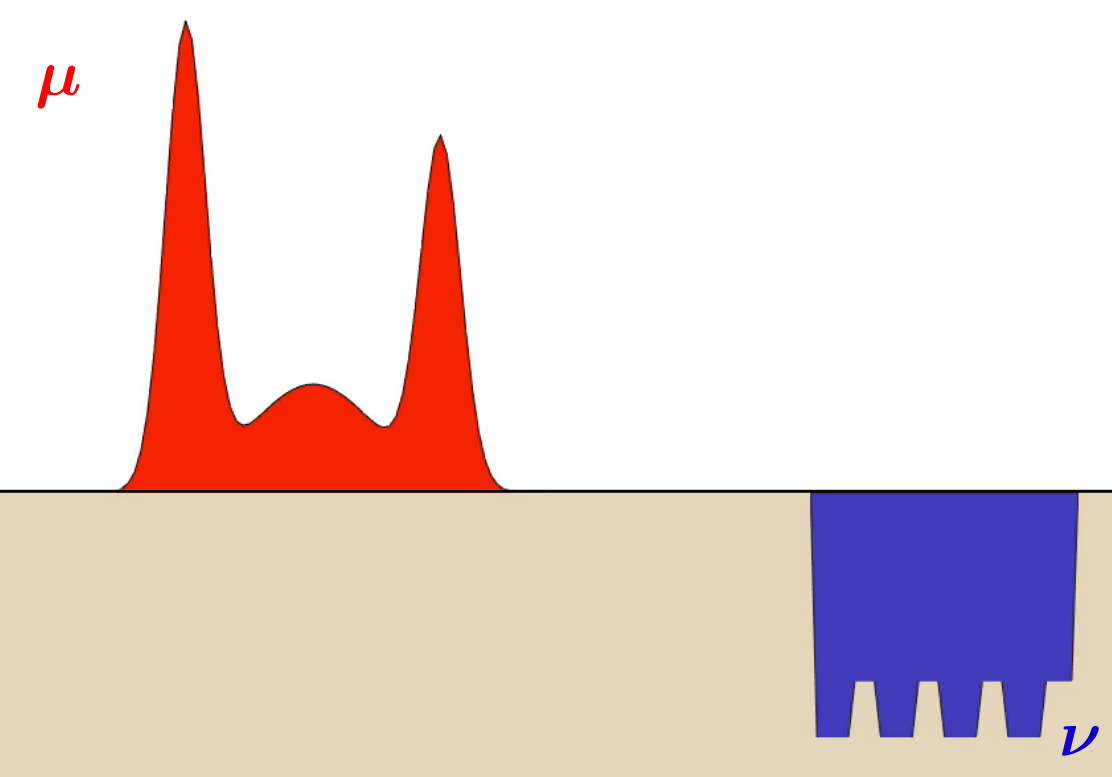
\includegraphics[width=0.5\textwidth]{img/transporte/montanas-arena-pozo.png}
    \caption{Representación de la pila de arena, representada en rojo por la medida $\mu$, y el pozo, representada en azul por la medida $\nu$. Imagen obtenida de \cite{cuturi2017primer}.}
    \label{fig:montanas-arena-pozo}
\end{figure}

Utilizando términos matemáticos, este problema se formula de la siguiente manera: sea un espacio de arena $\cX$, un espacio de pozo $\cY$, y una función de costo $c: \cX \times \cY \to \R$, donde la función de costo representa el \emph{esfuerzo} necesario para transportar una unidad de arena del punto $x \in \cX$ a una posición en el pozo $y \in \cY$. La distribución de la arena se describe mediante una medida $\mu \in \ProbSpace[\cX]$, mientras que la forma del pozo se caracteriza mediante una medida $\nu \in \ProbSpace[\cY]$.

La \emph{decisión} sobre cómo transportar la arena se representa mediante una función $T: \cX \to \cY$, que asigna a cada punto $x \in \cX$ una posición $T(x) \in \cY$ en el pozo. El ``esfuerzo total'' que el trabajador debe realizar corresponde a ``sumar'' todos los costos asociados al transporte de la arena desde $x$ hasta la posición correspondiente en el pozo $T(x)$. Más formalmente, el \emph{costo total} de transportar la arena al pozo se obtiene integrando el costo $c$ sobre todo el espacio de arena $\cX$:
\begin{equation}\label{eq:costoTotalTransporteMonge}
    C(T) \eqdef \int_{\cX} c(x, T(x)) \dmu[x].
\end{equation}

Una primera propiedad que se debe exigir a la función $T$ es que preserve la masa total de la arena. Es decir, para cualquier conjunto $B \subseteq \cY$ que represente una región en el pozo con volumen $\nu(B)$, se requiere que el volumen de arena asignado a la región $B$ por la ``decisión'' $T$ sea exactamente el mismo volumen que se rellenará en $B$. La cantidad de arena que ocupará $B$ bajo la ``decisión'' $T$ se expresa como $\left\{ x \in \cX : T(x) \in B \right\} = T^{-1}(B)$, y por lo tanto, la condición de preservación de masa implica que $\mu(T^{-1}(B)) = \nu(B)$ para todo $B \subseteq \cY$.

\begin{figure}[H]
    \centering
    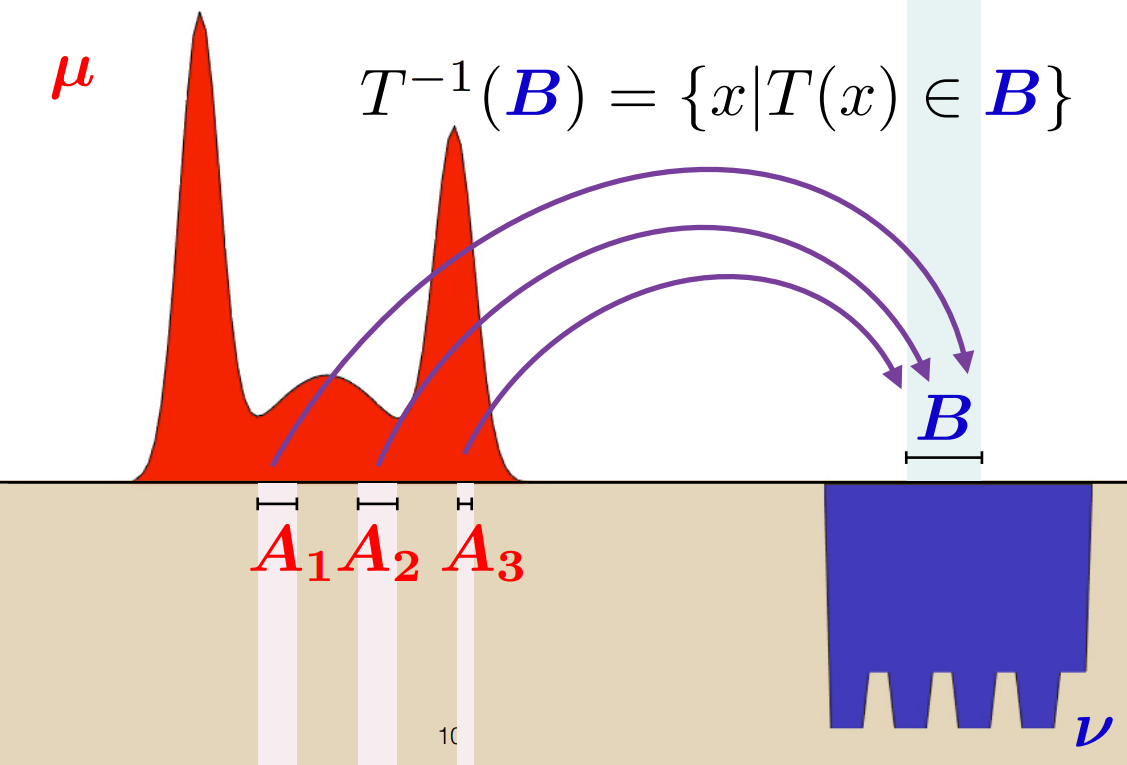
\includegraphics[width=0.5\textwidth]{img/transporte/preservacion-masa.png}
    \caption{Representación de como la función $T$ ha de preservar la masa total de la arena. Imagen obtenida de \cite{cuturi2017primer}.}
    \label{fig:preservacion-masa}
\end{figure}

Esta condición se ilustra gráficamente en la Figura~\ref{fig:preservacion-masa} y se formula de manera más precisa mediante la definición del operador \textit{push-forward}:

\begin{definition}[Operador \textit{push-forward}]\label{def:operador-push-forward}
    Sean $\mu \in \ProbSpace[\cX] $, $\nu \in \ProbSpace[\cY] $ dos medidas de probabilidad y
    sea una función medible $T:\cX \to \cY$. Se define el \emph{operador push-forward} de $T$ como la aplicación $\Tpf:\ProbSpace[\cX] \to \ProbSpace[\cY]$ que satisface la siguiente relación:
    \begin{equation}
        \label{eq:pushForward}
        \Tpf \mu(B) \eqdef \mu (T^{-1}(B)) = \nu(B),\quad \forall B \subseteq \cY,\ \nu\text{-medible}.
    \end{equation}
    Equivalentemente, para toda función $\nu$-integrable $g$,
    el operador push-forward satisface
    \begin{equation}
        \label{eq:pushForwardIntegral}
        \int_{\cY} g(y) \; \nu (\dd y) = \int_{\cX} g(T(x)) \; \mu (\dd x).
    \end{equation}
    En este caso, se dice que la función $T$ es un \emph{cambio de variables desde $\mu$ hasta $\nu$}.
\end{definition}

Ahora que se disponen de todas las herramientas matemáticas necesarias, se puede definir este problema como el de encontrar una función $T$, que representa la manera de transportar la arena al pozo, tal que minimice el costo total de transporte $C(T)$, sujeto a la condición de que la masa total de la arena sea preservada. De manera más formal:

\begin{definition}[Problema de Monge \cite{monge1781memoire}]
    Dadas dos medidas $\mu \in \ProbSpace[\cX]$ y $\nu \in \ProbSpace[\cY]$ y una función de coste $c : \cX \times \cY \to \R$, el \emph{problema de transporte óptimo de Monge} se define como el problema de encontrar una función medible $T: \cX \to \cY$ que minimice el costo total de transporte $C(T)$. Es decir, que minimice la siguiente expresión:
    \begin{equation}
        \label{eq:problemaTransporteMonge}
        \inf_{T: \Tpf \mu = \nu} \int_{\cX} c(x, T(x)) \dmu[x].
    \end{equation}
    A aquella función $T$ que resuelva este problema se le llamará \emph{función de transporte} o \emph{mapa de transporte}, y se denotará por $T_{\mu \to \nu}$, o simplemente $T$ si es que no existe confusión.
\end{definition}

El problema introducido por Monge \cite{monge1781memoire} es, en general, considerablemente difícil. Esto se debe principalmente a que el conjunto de mapas de transporte $\left\{ T : \Tpf \mu = \nu \right\}$ es intratable. Además, puede suceder que no exista ninguna solución, o en el caso de que exista, esta podría no ser única, como veremos en los siguientes ejemplos:

\begin{example}\label{ex:problemaDeMongeSinSolucion}
    Consideremos $\cX = \left\{ -1, 1 \right\}$, $\cY = \left\{ 0 \right\}$, con $\mu = \frac{1}{2} \delta_{-1} + \frac{1}{2} \delta_{1}$ y $\nu = \delta_0$. En este caso, la función de transporte óptima que minimiza \eqref{eq:problemaTransporteMonge} es
    \begin{align*}
        T_{\mu \to \nu}(-1) & = 0 & T_{\mu \to \nu}(1) & = 0.
    \end{align*}
    Sin embargo, es importante destacar que no existe un transporte óptimo $T_{\nu \to \mu}$ que transporte la masa de $\nu$ a $\mu$. Esto se debe a que la masa de $\nu$ está concentrada en un solo punto, mientras que la masa de $\mu$ está distribuida en dos puntos. No es posible ``dividir'' la masa debido a la naturaleza determinista de los mapas de transporte. Este ejemplo ilustra un caso en el que el problema de Monge no tiene solución.
\end{example}

\begin{example}\label{ex:problemaDeMongeMultipleSolucion}
    Consideremos ahora $\cX = \left\{ (1, 1), (-1, -1) \right\}$, $\cY = \left\{ (-1, 1), (1, -1) \right\}$, con $\mu = \frac{1}{2} \delta_{(1, 1)} + \frac{1}{2} \delta_{(-1, -1)}$ y $\nu = \frac{1}{2} \delta_{(-1, 1)} + \frac{1}{2} \delta_{(1, -1)}$. Este ejemplo correspondería a uno en que los puntos de $\cX$ y $\cY$ forman un cuadrado. En este escenario, se observa que existen dos funciones de transporte óptimo $T^1_{\mu\to\nu}$ y $T^2_{\mu\to\nu}$ que minimizan \eqref{eq:problemaTransporteMonge}. Estas funciones se expresan como:
    \begin{align*}
        T^1_{\mu\to\nu}(1, 1) & = (1, -1) & T^1_{\mu\to\nu}(-1, -1) & = (-1, 1)  \\
        T^2_{\mu\to\nu}(1, 1) & = (-1, 1) & T^2_{\mu\to\nu}(-1, -1) & = (1, -1).
    \end{align*}
    Este ejemplo muestra que, en ciertos casos, el problema de Monge puede tener más de una solución.
\end{example}



%   \begin{remark}
% 	  \label{remark:problemaTransporteMongeDiscreto}
% 	  Cuando las medidas $\mu$ y $\nu$ son discretas, es decir, se representan de la siguiente manera:
% 	  \begin{align}
% 		  \mu & = \sum_{i=1}^{n} a_i \delta_{x_i}, &
% 		  \nu & = \sum_{j=1}^{m} b_j \delta_{y_j},
% 	  \end{align}
% 	  donde $a \in \Simplex[n]$, $b \in \Simplex[m]$, $x_1,\ldots, x_n  \in \cX$, $y_1,\ldots, y_m  \in \cY$, entonces el problema de transporte óptimo se puede representar de la siguiente manera:
% 	  \begin{equation}
% 		  \label{eq:problemaTransporteDiscreto}
% 		  \inf_{T: T(x_i) = y_j} \sum_{i=0}^{n} a_i c(x_i, T(x_i)).
% 	  \end{equation}

\subsection{El problema de Kantorovich}  % MARK: El problema de Kantorovich

Como se pudo apreciar en los Ejemplos \ref*{ex:problemaDeMongeSinSolucion} y \ref*{ex:problemaDeMongeMultipleSolucion}, el problema de Monge no siempre tiene solución y, en caso de tenerla, puede que esta no sea única. Motivado por esto, Kantorovich \cite{kantorovich1942translocation} propuso una formulación relajada del problema de Monge.

La idea principal de Kantorovich es relajar la naturaleza determinista del mapa de transporte, es decir, el hecho de que la masa de un punto $x$ sea transportada a un único punto $T(x)$, como se ilustró en el Ejemplo~\ref{ex:problemaDeMongeSinSolucion}. En cambio, Kantorovich propone que la masa de un punto $x$ puede ser potencialmente transportada a múltiples destinos.

Para representar formalmente esta idea, consideremos una medida de probabilidad $\pi \in \ProbSpace[\cX \times \cY]$. En este contexto, la cantidad $\pi(A \times B)$ representaría la cantidad de arena transportada desde el conjunto $A \subseteq \cX$ hasta la región del pozo representada por el conjunto $B \subseteq \cY$. La masa total enviada desde $A$ sería $\pi(A \times \cY)$, y la masa total enviada a $B$ sería $\pi(\cX \times B)$. En este contexto, $\pi$ estaría preservando la masa total si, y solo si, se cumple que
\begin{align*}
    \pi(A \times \cY) & = \mu(A), \quad \forall A \subset \cX \text{ medible;} \\
    \pi(\cX \times B) & = \nu(B),\quad \forall B \subset \cY \text{ medible.}
\end{align*}
Las medidas $\pi$ que cumplen esta condición se conocen como \emph{couplings}, y se pueden definir de manera más formal de la siguiente manera:\FM{Quizás no sea necesaria la definición si lo definí en esta línea.}

\begin{definition}[Coupling]
    Sean $(\cX, \mu)$ y $(\cY, \nu)$ dos espacios de probabilidad. Un \emph{coupling} entre $\mu$ y $\nu$ es una medida de probabilidad $\pi \in \ProbSpace[\cX \times \cY]$ tal que sus proyecciones marginales sean $\mu$ y $\nu$, es decir, que cumpla que
    \begin{equation}
        \label{eq:coupling}
        \pi(A \times \cY) = \mu(A), \quad \pi(\cX \times B) = \nu(B), \quad \forall A \subseteq \cX, B \subseteq \cY \text{ medibles}.
    \end{equation}
    Al conjunto de couplings entre $\mu$ y $\nu$ se le denotará por $\Cpl(\mu, \nu)$. Usualmente se les llama a $\mu$ y $\nu$ como la primera y segunda \emph{distribución marginal}, o simplemente \emph{marginales} de $\pi$.
\end{definition}

Al igual que en el problema de Monge, se puede definir el costo total de transporte de un coupling $\pi \in \Cpl(\mu, \nu)$, utilizando una función de coste $c: \cX \times \cY \to \R$:
\begin{equation}
    C(\pi) = \int_{\cX \times \cY} c(x, y) \dpi (\dd x, \dd y).
\end{equation}

Y utilizando esta definición, se puede definir el problema de transporte óptimo de Kantorovich de forma análoga al problema de Monge:
\begin{definition}[Problema de Kantorovich \cite{kantorovich1942translocation}]
    Dadas dos medidas $\mu \in \ProbSpace[\cX]$ y $\nu \in \ProbSpace[\cY]$ y una función de coste $c: \cX \times \cY \to \R$, el \emph{problema de transporte óptimo de Kantorovich} se define como el problema de encontrar un coupling $\pi \in \Cpl(\mu, \nu)$ que minimice el costo total de transporte, es decir, que minimice la siguiente expresión:
    \begin{equation}
        \label{eq:problemaTransporteKantorovich}
        \inf_{\pi \in \Cpl(\mu, \nu)} \int_{\cX \times \cY} c(x, y) \dpi (\dd x, \dd y).
    \end{equation}
    Al conjunto de couplings que resuelven este problema se le llama \emph{planes de transporte} o \emph{couplings óptimos}, y un coupling que minimice este problema se denotará por $\pi_{\mu \to \nu}$, o simplemente $\pi$ si es que no existe confusión.
\end{definition}


En diferencia con el problema de Monge, el problema de Kantorovich siempre tiene solución, si es que $(\cX, \cY)$ son espacios compactos y $c$ es continuo. En efecto, $\Cpl(\mu, \nu)$ es compacto para la topología débil de las medidas,  $\pi \mapsto \int c\dd{\pi}$ es una función continua para esta topología, y la restricción $\pi\in\Cpl(\mu, \nu)$ es no vacía (la medida producto $\mu \otimes \nu$ pertenece a $\Cpl(\mu, \nu)$). Como se busca un ínfimo en un compacto de una función continua, se sigue que existe un coupling óptimo $\pi_{\mu \to \nu}$ que resuelve \eqref{eq:problemaTransporteKantorovich}.

\begin{figure}[H]
    \centering
    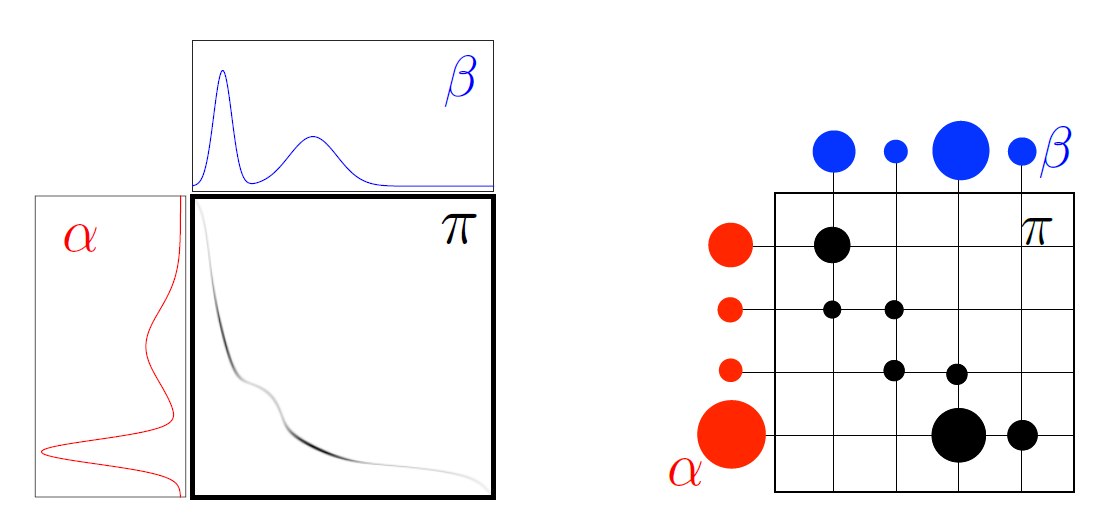
\includegraphics[width=0.7\textwidth]{img/transporte/coupling-example.png}
    \caption{Izquierda: coupling óptimo entre dos medidas 1-D continuas con densidad. El coupling está localizado a lo largo del grafo del mapa de transporte óptimo $(x, T(x))$. Derecha: coupling óptimo entre dos medidas discretas. El radio del disco negro es proporcional a la masa transportada en esa coordenada. Imagen obtenida de \cite{peyre2019computational}.
        \label{fig:coupling-example}}
\end{figure}

Continuando con los ejemplos \ref*{ex:problemaDeMongeSinSolucion} y \ref*{ex:problemaDeMongeMultipleSolucion}, podemos encontrar el coupling óptimo para cada uno de estos problemas:

\begin{example}
    Sean los espacios $\cX$ y $\cY$ y las medidas $\mu$ y $\nu$ como en el Ejemplo~\ref*{ex:problemaDeMongeSinSolucion}. En este caso, el coupling óptimo entre $\mu$ y $\nu$ corresponde a:
    \begin{align*}
        \pi_{\mu \to \nu}\left\{ (-1, 0) \right\} & = \frac{1}{2} & \pi_{\mu \to \nu}\left\{ (1, 0) \right\} & = \frac{1}{2}.
    \end{align*}
    Del mismo modo, el coupling óptimo entre $\nu$ y $\mu$ corresponde a:
    \begin{align*}
        \pi_{\nu \to \mu}\left\{ (0, -1) \right\} & = \frac{1}{2} & \pi_{\nu \to \mu}\left\{ (0, 1) \right\} & = \frac{1}{2}.
    \end{align*}

\end{example}

\begin{example}
    Del mismo modo, Sean los espacios $\cX$ y $\cY$ y las medidas $\mu$ y $\nu$ como en el Ejemplo~\ref*{ex:problemaDeMongeMultipleSolucion}. En este caso, el coupling óptimo entre $\mu$ y $\nu$ corresponde a:
    \begin{align*}
        \pi_{\mu \to \nu}\left\{ \qty\Big((1, 1), (-1, 1)) \right\}   & = \frac{1}{4} & \pi_{\mu \to \nu}\left\{ \qty\Big((1, 1), (1, -1)) \right\}   & = \frac{1}{4}  \\
        \pi_{\mu \to \nu}\left\{ \qty\Big((-1, -1), (-1, 1)) \right\} & = \frac{1}{4} & \pi_{\mu \to \nu}\left\{ \qty\Big((-1, -1), (1, -1)) \right\} & = \frac{1}{4}.
    \end{align*}

\end{example}

Para finalizar esta sección, una pregunta que surge naturalmente es: ¿Cuál es relación entre los problemas de Monge y Kantorovich? ¿Si encuentro una solución para el problema de Kantorovich, puedo tener una solución para el problema de Monge? La respuesta es que, bajo algunas condiciones particulares, estos dos problemas están estrechamente relacionados, como lo establece el teorema de Brenier \cite{brenier1991polar}:

\begin{theorem}[Brenier \cite{brenier1991polar}]
    Sea $\cX = \cY = \R^d$, $c(x, y) = \|x - y\|^2$, $\mu\in \ProbSpace[\cX] $ y $\nu\in \ProbSpace[\cY] $. Si al menos una de las dos medidas (que s.p.g. supondremos que es $\mu$) tiene densidad con respecto a la medida de Lebesgue, entonces el plan de transporte óptimo $\pi$ es único y esta soportado en el grafo $(x, T(x))$ de un mapa de transporte óptimo $T:\cX \to \cY$. Esto significa que el plan de transporte es $\pi = \pf{(\id, T)}\mu$, y cumple la siguiente ecuación:
    \begin{equation}
        \forall h \in \cC(\cX \times \cY),\quad \int_{\cX\times\cY}^{} h(x, y) \dpi (\dd x, \dd y) = \int_{\cX}^{} h(x, T(x)) \dmu[x].
    \end{equation}
    Más aún, el mapa de transporte óptimo $T$ está únicamente definido como el gradiente de una función convexa $\phi$, i.e. $T(x) = \grad \phi(x)$, donde $\phi$ es la única función convexa (salvo una constante aditiva) tal que $\pf{(\grad \phi)} \mu = \nu$.

    A aquellos mapas de transporte $\pi\in\Cpl(\mu, \nu)$ que se encuentran definidos por $\pi = \pf{(\id, T)} \mu$, para algún mapa de transporte $T$, se les llama \emph{mapas deterministas}, pues cumple con la propiedad de que si $(X, Y) \sim \pi$, entonces $Y$ queda determinado por $Y = T(X)$.
\end{theorem}

\begin{proof}
    Se puede encontrar una demostración de este teorema en \cite[p. 27]{peyre2019computational}
\end{proof}

\FM[inline]{Pensaba en agregar otra sección con la interpretación probabilista, como en \cite[\S 1.2]{panaretos2020invitation}}

\section{La Distancia y el Espacio de Wasserstein}\label{sec:la-distancia-y-el-espacio-de-Wasserstein}  % MARK: La Distancia y el Espacio de Wasserstein

Como se revisó en la sección anterior, cuando se considera el problema de Kantorovich, este problema usualmente tiene solución.
Si es que se considera $(\cX, \dist)$ un espacio métrico, se podría interpretar la distancia como una forma de representar el costo de transportar la masa de un punto $x$ a un punto $y$.
Pero una vez que se hace esto, naturalmente surge la pregunta: ¿Qué propiedades pueden surgir al considerar la distancia como una función de coste?
Esta sección responde a estas preguntas. Para ello, se empieza definiendo la distancia de Wasserstein, para luego revisar algunas de sus propiedades.
Esta sección estará basada en la Sección 6 del libro de Villani \cite{villani2009optimal}.
\FM{Incluir subsections para la distancia, espacio, y convergencia débil?}

\begin{definition}[La distancia de Wasserstein]\label{def:distanciaWasserstein}
    Sea $(\cX, \dist)$ un espacio Polaco y sea $p \geq 1$. Para dos medidas $\mu, \nu$ sobre $\cX$, la distancia de Wasserstein de orden $p$ entre $\mu$ y $\nu$ es definida por medio de la fórmula
    \begin{equation}
        \label{eq:distanciaWasserstein}
        \Wasserstein[p]{\mu}{\nu}  \eqdef \left( \inf_{\pi \in \Cpl(\mu, \nu)} \int_{\cX \times \cX} \dist(x, y)^{p} \dpi (\dd x, \dd y) \right)^{\frac{1}{p}}.
    \end{equation}

\end{definition}

\begin{example}
    $\Wasserstein[p]{\delta_x}{\delta_y} = \dist(x, y)$. Notemos que en este ejemplo, se puede interpretar que la distancia de Wasserstein metriza el ``esfuerzo'' de llevar la masa del punto $x$ al punto $y$, y que además, es independiente del valor de $p$.
\end{example}

Como el nombre de $W_p$ puede sugerir, esta es una distancia sobre medidas de probabilidad. Sin embargo, si esta es definida sobre todo el espacio $\ProbSpace[\cX]$, entonces puede tomar valores de $+\infty$, de forma que en estricto rigor, $W_p$ aún no puede ser considerada una distancia.
Para remediar este problema, se definirá un espacio de medidas de probabilidad en el que la distancia de Wasserstein tome valores finitos.

\begin{definition}[El espacio de Wasserstein]
    Con los mismos supuestos que en la Definición \ref{def:distanciaWasserstein}, se define el espacio de Wasserstein de orden $p$ por medio de
    \begin{equation}
        \WassersteinSpace[p]{\cX} \eqdef \left\{
        \mu \in \ProbSpace[\cX] \colon \int_{\cX} \dist(x, x_0)^{p} \dmu[x] < \infty
        \right\},
    \end{equation}
    para algún punto fijo $x_0 \in \cX$. De esta forma, $W_p$ define una distancia (finita) sobre $\WassersteinSpace[p]{\cX}$.
\end{definition}

En palabras simples, el espacio de Wasserstein de orden $p$ es el conjunto de medidas de probabilidad en $\cX$ cuyo momento de orden $p$ es finito.\FM{Será necesario este último comentario?}

En \cite[p. 94]{villani2009optimal} se puede encontrar una demostración de que $\WassersteinSpace[p]{\cX}$ satisface con los tres axiomas de una distancia. Es más, se puede demostrar que $\WassersteinSpace[p]{\cX}$ puede heredar varias propiedades del espacio base $\cX$, como lo presenta el siguiente teorema:
\begin{theorem}[Topología del espacio de Wasserstein \cite{villani2009optimal}]
    \label{thm:espacioWassersteinEsMetrico}
    Si $(\cX, \dist)$ es un espacio Polaco, entonces el espacio de Wasserstein $\WassersteinSpace[p]{\cX} $, metrizado por la distancia de Wasserstein $W_p$, es también un espacio Polaco.
\end{theorem}

\begin{proof}
    Revisar la demostración del Teorema 6.18 en \cite[p. 105]{villani2009optimal}
\end{proof}

\FM[inline]{Desde aquí en adelante, creo que se puede mover a otras secciones, si es que se necesita}

A partir de ahora, se asumirá que el espacio $\WassersteinSpace[p]{\cX} $ siempre estará equipado con su respectiva distancia $W_p$.\FM{Creo que esta línea no es del todo necesaria}


\begin{remark}
    A través de la desigualdad de Hölder, se puede demostrar que para $p \leq q$, se tiene que $\Wasserstein[p]{\mu}{\nu} \leq \Wasserstein[q]{\mu}{\nu}$, para toda $\mu, \nu \in \WassersteinSpace[p]{\cX}$. Y por tanto, las topologías inducidas por las distancias de Wasserstein se van encajonando.\FM{Esta observación no es tan necesaria para esta primera parte de preliminares}

    En particular, la distancia de Wasserstein de orden 1, es la más débil de todas. Como norma general, la distancia $W_1$  es la más flexible y fácil de acotar, mientras que la distancia $W_2$ posee mejores propiedades geométricas, pero es más difícil de trabajar.
\end{remark}

\FM[inline]{Toda la parte de la convergencia débil la moveré cuando pase a ver las WGANs}
Vista la distancia y el espacio de Wasserstein, se presentará una caracterización de convergencia en este espacio. Para ello, se definirá la convergencia débil entre medidas de probabilidad.

\begin{definition}[Convergencia Débil]
    Sea $(\cX, \dist)$ un espacio Polaco y sea $p \geq 1$. Se dice que una sucesión de medidas de probabilidad $(\mu_n)_{n \in \N} \subset \WassersteinSpace[p]{\cX} $ converge débilmente a $\mu \in \WassersteinSpace[p]{\cX}$ si
    \begin{equation}
        \forall \phi \in \ContBoundedSpace[\cX], \quad \int_{\cX} \phi(x) \dd{\mu_n(x)} \to \int_{\cX} \phi(x) \dmu[x].
    \end{equation}
    y lo denotaremos por $\mu_n \wto \mu$.
\end{definition}

\begin{note}
    Intuitivamente, que una sucesión de medidas de probabilidad converjan débilmente a una medida $\mu$ significa que es la forma ``más fácil'' que tiene la sucesión de converger a $\mu$.
\end{note}

\begin{theorem}[La Distancia de Wasserstein Metriza la Convergencia Débil]
    Sea $(\cX, \dist)$ un espacio Polaco y sea $p \geq 1$. Entonces, la distancia de Wasserstein $W_p$  metriza la convergencia débil en $\WassersteinSpace[p]{\cX}$.
\end{theorem}

\begin{remark}
    En otras palabras, si $(\mu_n)_{n\in\N}$ es una sucesión de medidas de probabilidad en $\WassersteinSpace[p]{\cX}$ y $\mu\in \WassersteinSpace[p]{\cX} $ otra medida, entonces $\mu_n \wto \mu$ si y sólo si $\Wasserstein[p]{\mu_n}{\mu} \to 0$.
\end{remark}

\begin{example}
    Consideremos las siguientes distancias y divergencias entre medidas de probabilidad:
    \begin{gather*}
        \TV{\mu}{\nu} \eqdef \sup_{A \subseteq \cX} \abs{\mu(A) - \nu(A)}, \\
        \KL{\mu}{\nu} \eqdef \int_{\cX} \log\left(\dv{\mu}{\nu}(x)\right) \dmu[x], \\
        \JS{\mu}{\nu} \eqdef \KL{\mu}{\frac{\mu + \nu}{2}} + \KL{\nu}{\frac{\mu + \nu}{2}},
    \end{gather*}
    donde la primera es la distancia total variación, la segunda es la divergencia de Kullback-Leibler, y la tercera es la divergencia de Jensen-Shannon.

    Si consideramos $\delta_\theta$ y $\delta_0$ medidas de Dirac centradas en $\theta$ y $0$ respectivamente, entonces se puede demostrar que
    \begin{align*}
        \Wasserstein[1]{\delta_\theta}{\delta_0} & = |\theta|                            &
        \TV{\delta_\theta}{\delta_0}             & = \begin{cases}
                                                         1 & \text{si } \theta \neq 0 \\
                                                         0 & \text{si } \theta = 0
                                                     \end{cases}          \\
        \KL{\delta_\theta}{\delta_0}             & = \begin{cases}
                                                         +\infty & \text{si } \theta \neq 0 \\
                                                         0       & \text{si } \theta = 0
                                                     \end{cases} &
        \JS{\delta_\theta}{\delta_0}             & = \begin{cases}
                                                         \log(2) & \text{si } \theta \neq 0 \\
                                                         0       & \text{si } \theta = 0
                                                     \end{cases}
    \end{align*}
    Entonces, si tomamos $\theta = \frac{1}{n} $ y dejamos que $n \to \infty$, se tiene que $\Wasserstein[1]{\delta_\theta}{\delta_0} \to 0$, pero el resto de distancias y divergencias no convergen a 0.
    Por tanto, se puede notar que la distancia de Wasserstein es la única que es capaz de distinguir entre medidas de probabilidad que no tienen soporte en el mismo punto, gracias a que metriza la convergencia débil.
\end{example}

\section{El Baricentro de Wasserstein}\label{sec:el-baricentro-de-Wasserstein-Bayesiano}  % MARK: El Baricentro de Wasserstein

Esta sección presenta el concepto de baricentro de Wasserstein, el cual es una generalización del concepto de promedio para medidas de probabilidad. Este concepto es clave para definir el baricentro de Wasserstein Bayesiano, el cual es el principal objeto de estudio de esta tesis. Para ello, se empieza revisando el concepto de media de Fréchet, luego se define el baricentro de Wasserstein, se revisan técnicas de cálculo de baricentros de población, y finalmente se define el baricentro de Wasserstein Bayesiano. La escritura de esta sección se basa en ejemplos de la Sección 3 de Panaretos y Zemel \cite{panaretos2020invitation} y en definiciones de la Sección 9.2 de Peyré y Cuturi \cite{peyre2019computational}.

\subsection{La Media de Fréchet}\label{ssec:la-media-de-Frechet}  % MARK: La Media de Fréchet
%   En esta sección se revisará el concepto de media de Fréchet, el cual es una generalización de la noción de promedio para espacios métricos. Este concepto será clave para definir el baricentro de Wasserstein.

\begin{definition}[Funcional y Media de Fréchet \cite{frechet1948elements}]
    Sea $(\cX, \dist)$ un espacio Polaco. Sean $(x_{i})_{i=1}^{n}\in\cX^n$ puntos en $\cX$ y sean $(\gamma_{i})_{i=1}^{n}\in\R_+^n$ los pesos asociados a esos puntos. Para cada $p\in\cX$, se define el \emph{funcional de Fréchet} por
    \begin{equation}
        \label{eq:funcionalFrechet}
        \Psi(p) \eqdef \sum_{i=1}^{n} \gamma_i \dist(p, x_i)^2.
    \end{equation}
    Y, en caso de que exista un punto $\bar x \in \cX$ que minimice el funcional $\Psi$, entonces este se definirá como la \emph{media de Fréchet} de los puntos $(x_{i})_{i=1}^{n}$. Es decir, es aquel punto tal que minimiza el siguiente problema:
    \begin{equation}
        \label{eq:mediaFrechet}
        \bar x \eqdef \argmin_{p \in \cX} \sum_{i=1}^{n} \gamma_i \dist(p, x_i)^2.
    \end{equation}
\end{definition}

\begin{example}\label{ex:baricentro-triangulo}
    Tomemos $x_1, x_2, x_3 \in \R^2$ tres puntos en el plano, formando un triángulo. Si se define el promedio (o el \textit{baricentro}, en el contexto de la geometría) de estos puntos por $\bar x = \frac{1}{3} (x_1 + x_2 + x_3)$, entonces se comprueba fácilmente que este es el único que minimiza el funcional de Fréchet:
    \begin{equation}
        F(p) = \frac{1}{3} \sum_{i=1}^{3} \|p - x_i\|^2,
    \end{equation}
    puesto que este funcional se descompone de la siguiente manera:
    \begin{equation}
        F(p) = F(\bar x) + \|p-\bar x\|^2.
    \end{equation}
    Con este ejemplo, se aprecia que la media de Fréchet generaliza la noción de promedio.
\end{example}

La razón por la que resulta interesante estudiar este concepto, es que únicamente utiliza nociones métricas, desligándose de nociones vectoriales. Como se vió en el Ejemplo~\ref{ex:baricentro-triangulo}, el promedio $\bar x$ utiliza conceptos vectoriales (suma y ponderación de vectores) mientras que la media de Fréchet utiliza nociones métricas (a través de la distancia $\dist(x, y) = \|x - y\|$), resultando en el mismo promedio.

Lo interesante de la media de Fréchet, es que este concepto es mucho más general, pues la media depende ahora de la distancia que se esté utilizando.


\subsection{El Baricentro de Wasserstein}\label{ssec:el-baricentro-de-Wasserstein}  % MARK: El Baricentro de Wasserstein

Como se vió en la sección anterior, la media de Fréchet permite definir una noción de promedio para espacios métricos. Además, el Teorema~\ref{thm:espacioWassersteinEsMetrico} establece que si $(\cX, \dist)$ es un espacio Polaco, entonces $(\WassersteinSpace[p]{\cX}, W_p)$ es un espacio Polaco, y en particular, un espacio métrico. Por tanto, se puede definir su respectivo ``promedio'' utilizando la media de Fréchet:

% \newacronym{wb}{WB}{baricentro de Wasserstein}

% MARK: Baricentro de Wasserstein
\begin{definition}[Baricentro de Wasserstein \cite{agueh2011barycenters}]\label{def:baricentroWasserstein}
    Sean $(\mu_{i})_{i=1}^{n}$ medidas en $\WassersteinSpace[p]{\cX} $ y sean $(\gamma_{i})_{i=1}^{n} \in \R_+^n$ sus pesos asociados. El \emph{baricentro de Wasserstein} se define por medio de
    \begin{equation}
        \bar \mu \eqdef \arginf_{\nu \in \WassersteinSpace[p]{\cX} } \sum_{i=1}^{n} \gamma_i \Wasserstein[p]{\nu}{\mu_i}^p.
    \end{equation}

\end{definition}

Un ejemplo de distintos baricentros, variando los pesos $(\gamma_i)_i$, se observa en la Figura~\ref{fig:baricentro-Wass-3d}.

\begin{figure}[H]
    \centering
    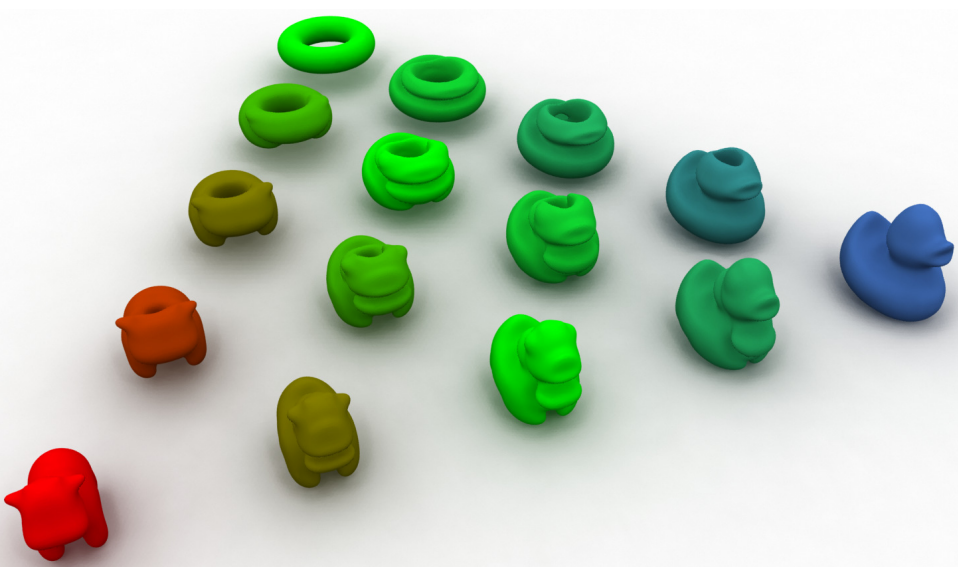
\includegraphics[width=0.5\textwidth]{img/transporte/baricentro-Wass-3d.png}
    \caption{Baricentro entre tres figuras en 3 dimensiones, donde se variaron los pesos $\gamma_i$ de forma bilineal. Imagen obtenida de \cite{solomon2015convolutional}.}
    \label{fig:baricentro-Wass-3d}
\end{figure}


% MARK: Interpolación geodésica
Cabe destacar que para el caso en donde se considera $n = 2$, el baricentro de Wasserstein recibe un nombre especial: \textit{interpolación geodésica de McCann}, el cuál se define a continuación:

\begin{definition}[Interpolación Geodésica de McCann \cite{mccann1997convexity}]
    Sea $\mu_0, \mu_1 \in \WassersteinSpace[p]{\cX} $ dos medidas y $t \in [0, 1]$ el parámetro de interpolación. La \emph{$t$-interpolación geodésica de McCann} (o simplemente, \emph{interpolación geodésica}) se define por medio de:
    \begin{equation}\label{eq:interpolacion-geodesica}
        \mu_t \eqdef \arginf_{\mu \in \WassersteinSpace[p]{\cX} } (1-t) \cdot \Wasserstein[p]{\mu_0}{\mu}^p + t \cdot \Wasserstein[p]{\mu}{\mu_1}^p.
    \end{equation}
    El parámetro $t$ controla la cantidad de influencia de cada medida en el baricentro, en particular, para $t = 0$ se recupera $\mu_0$, y para $t = 1$ se recupera $\mu_1$.
\end{definition}


%  En este caso, se consideran dos medidas $\mu_0, \mu_1 \in \WassersteinSpace[p]{\cX} $ y se define el baricentro de Wasserstein con pesos $\gamma = (1 - t, t)$, para $t \in [0, 1]$:
% \begin{equation}\label{eq:interpolacion-geodesica}
%     \mu_t \eqdef \arginf_{\mu \in \WassersteinSpace[p]{\cX} }  (1-t) \Wasserstein[p]{\mu_0}{\mu}^p + t \Wasserstein[p]{\mu}{\mu_1}^p .
% \end{equation}


\FM[inline]{Se podría agregar el teorema que dice que el baricentro existe y es único, aunque no lo cacho mucho. Sé que es de Agueh y Carlier.}


Es posible generalizar aún más la noción de baricentro de Wasserstein a una colección infinita de medidas. Para esto, se considera una medida $\Gamma \in \ProbSpace[\ProbSpace ] $, que cumple el rol de los pesos $(\gamma_{i})_{i}$ en la definición anterior, lo que se formaliza en la siguiente definición:

\FM[inline]{Puede ser que en esta definición sea necesario incluir la definición utilizando el espacio de modelos como en el paper \cite{backhoff2022bayesian}}

% MARK: Baricentro de Población de Wasserstein
\begin{definition}[Baricentro de población de Wasserstein \cite{bigot2018characterization}]
    Sea $\Gamma \in \ProbSpace[\ProbSpace]$ una medida. El \emph{baricentro de población de Wasserstein} se define por medio de:
    \begin{equation}
        \label{eq:baricentroWassersteinGeneral}
        \bar \mu \eqdef \arginf_{\mu \in \ProbSpace} \int_{\ProbSpace} \Wasserstein[p]{\mu}{\nu}^p \dGamma[\nu].
    \end{equation}
\end{definition}

La razón por la que la definición anterior es una generalización, es que si se considera $\Gamma = \sum_{i=1}^{n} \gamma_i \delta_{\mu_i}$, entonces se recupera la primera definición. Además, cabe destacar que no es necesario especificar las medidas $(\mu_i)_{i=1}^{n}$, pues se encuentran implícitas en la medida $\Gamma$.

\begin{remark}
    Cabe destacar que en la definición anterior, el baricentro de Wasserstein es la medida que minimiza el promedio de las medidas generadas por $\Gamma$. De esta forma, la Ecuación \eqref{eq:baricentroWassersteinGeneral} se puede reescribir como:
    \begin{equation}
        \bar \mu \eqdef \arginf_{\mu \in \ProbSpace} \Big\{ \Exp_{\nu \sim \Gamma} \big[ \Wasserstein[p]{\mu}{\nu}^p \big] \Big\}.
    \end{equation}

\end{remark}

\subsection{El Descenson del Gradiente Estocástico en el Espacio de Wasserstein}\label{ssec:sgdw}  % MARK: SGDW El Descenso del Gradiente Estocástico sobre el Espacio de Wasserstein

Para calcular una estimación del baricentro de Wasserstein de una colección finita de medidas $\left\{ \mu_i \right\}_{i=1}^{n}$, existen múltiples algoritmos que se pueden utilizar. Por ejemplo, para el caso en que las medidas sean a soporte discreto, se puede deducir un problema de programación lineal \cite[ver Cap. 3]{peyre2019computational}, y resolver el problema de forma exacta \cite{bonneel2011displacement}, o utilizando una estimación de la solución por medio de métodos iterativos, como el algoritmo de Sinkhorn \cite{cuturi2013sinkhorn}. En el caso en que las medidas provengan de imágenes, se pueden utilizar métodos convolucionales, como en \cite{solomon2015convolutional} o en su versión mejorada e insesgada \cite{janati2020debiased}.

Sin embargo, para el caso en que la colección de medidas sean infinitas, como lo es en el caso del baricentro de población de Wasserstein, estos métodos no son aplicables. Por este motivo, en los trabajos \cite{rios2020contributions,backhoff2022stochastic,backhoff2022bayesian} proponen un algoritmo para encontrar este baricentro, por medio del Descenso del Gradiente Estocástico (SGD).

En los trabajos mencionados, se hacen los siguientes supuestos (que serán válidos sólo para esta sección de la tesis).

\begin{assumption}\label{assump:caso-particular-lebesgue}
    Se considera $p=2$, $\cX = \R^q$, $\dist$ la distancia Euclidiana, y $\lambda$ la medida de Lebesgue. Es más, con estos supuestos se tiene que $\Gamma \in \WassersteinSpace[2]{\WassersteinSpace[2,\mathrm{ac}]{\R^q} } $ y existe un espacio de modelos $\Models \subseteq \WassersteinSpace[2, \mathrm{ac}]{\R^q} $ para el cual $\Gamma$ es débilmente cerrado.
\end{assumption}

\begin{assumption}\label{assump:caso-particular-geodesicamente-convexo}
    $\Gamma$ tiene un espacio de modelos $W_2$-compacto: $K_\Gamma \subseteq \WassersteinSpace[2,\mathrm{ac}]{\R^q} $. Más aún, este conjunto es geodésicamente convexo: para cualesquiera $\mu_0, \mu_1 \in K_\Gamma$, la geodésica $\mu_t$ entre $\mu_0$ y $\mu_1$ está contenida en $K_\Gamma$.
\end{assumption}

\begin{assumption}\label{assump:caso-particular-esquema-paso-L1-L2}
    Para un esquema de paso\FM{Quizás podría definir qué es un esquema de paso.} $(\eta_k)_k \in [0, 1]^\N$, se asume que $\sum_{k=0}^{\infty} \eta_k = \infty$ y $\sum_{k=0}^{\infty} \eta_k^2 < \infty$.
\end{assumption}

\begin{definition}[Secuencia de SGDW \cite{backhoff2022stochastic,backhoff2022bayesian}]\label{def:sgdw}
    Dado $\mu_0 \in K_\Gamma$, $\tilde \mu_k \simiid \Gamma$ y $\eta_k > 0$ para $k \in\N$. Se define iterativamente la \textit{Secuencia de Descenso del Gradiente Estocástico sobre el Espacio de Wasserstein} (SGDW) por medio de:
    \begin{equation}
        \label{eq:sgdw}
        \mu_{k+1} \eqdef \pf{\qty\Big[
                (1 - \eta_k) \id + \eta_k T_{\mu_k \to \tilde \mu_k}
            ]} (\mu_k), \quad \text{para } k \in\N,
    \end{equation}
    donde $\eta_k \in [0, 1]$ es el tamaño de paso en la iteración $k$, y $T_{\mu_k \to \tilde \mu_k}$ es el transporte óptimo entre $\mu_k$ y $\tilde \mu_k$ como en la Definición~\ref{def:operador-push-forward}.
\end{definition}


% \begin{remark}
%     A pesar de que en la Definición~\ref{def:sgdw} se utilizó la notación de \textit{push-forward} (en donde se asume que $\mu_k$ y $\tilde \mu_k$ son absolutamente continuas con respecto a la medida de Lebesgue), basta con interpretar la notación de \textit{push-forward} como la interpolación geodésica entre $\mu_k$ y $\tilde \mu_k$, como se mencionó en \eqref{eq:interpolacion-geodesica}.

%     Con esta idea en mente, en la iteración $k$ de la Secuencia de SGDW se interpreta como si se estuviera transportando el $\eta_k\%$ de la masa de $\mu_k$ a $\tilde \mu_k$. Si $(\eta_k)_k$ es decreciente, entonces cada vez se mantiene más la forma de $\mu_k$.
% \end{remark}

\begin{remark}
    Gracias al supuesto de que $K_\Gamma$ es geodésicamente convexo, se tiene que $\mu_k \in K_\Gamma$ para toda $k \in\N$.
\end{remark}

El teorema principal que le da sentido a la definición anterior es el siguiente:

\begin{theorem}\label{thm:convergencia-sgdw}
    Se asumen los Supuestos~\ref{assump:caso-particular-lebesgue}, \ref{assump:caso-particular-geodesicamente-convexo}, \ref{assump:caso-particular-esquema-paso-L1-L2}, y que $\Gamma$ admite una única media de Karcher\FM{¿Será necesario incluir lo que es una media de Karcher? nunca lo ocupo directamente en el trabajo.}. Entonces la secuencia de SGDW $\left\{ \mu_k \right\}_k$ de la Ecuación~\eqref{eq:sgdw} converge c.s. al único 2-baricentro de Wasserstein $\bar \mu$ de $\Gamma$. Más aún, se tiene que $\bar \mu\in K_\Gamma$.
\end{theorem}

Además de la Secuencia de SGDW, en \cite{backhoff2022stochastic} se propone una versión de esta secuencia por lotes (o \textit{batched}, en inglés):

\begin{definition}[Secuencia de SGDW por lotes \cite{backhoff2022stochastic}]\label{def:bsgdw}
    Dado $\mu_0 \in K_\Gamma$, $\tilde \mu_k^{(1)}, \ldots, \tilde \mu_k^{(S_k)} \simiid \Gamma$ y $\eta_k > 0$ para $k \in\N$. Se define iterativamente la \textit{Secuencia de Descenso del Gradiente Estocástico sobre el Espacio de Wasserstein por lotes} (BSGDW) por medio de:
    \begin{equation}
        \label{eq:bsgdw}
        \mu_{k+1} \eqdef \pf{\qty[
                (1 - \eta_k) \id + \eta_k \frac{1}{S_k} \sum_{j=1}^{S_k} T_{\mu_k \to \tilde \mu_k^{(j)}}
            ]} (\mu_k) \quad \text{para } k \in\N,
    \end{equation}
    donde $\eta_k \in [0, 1]$ es el tamaño de paso, y $T_{\mu_k \to \tilde \mu_k^{(j)}}$ es el transporte óptimo entre $\mu_k$ y $\tilde \mu_k^{(j)}$ como en la Definición~\ref{def:operador-push-forward}.
\end{definition}

% \begin{remark}\label{rem:bsgdw}
%     En esta versión del SGDW por lotes, el operador \textit{push-forward} de la Ecuación~\eqref{eq:bsgdw} se interpreta como el baricentro de las medidas $(\mu_k, \tilde \mu_k^{(1)}, \ldots, \tilde \mu_k^{(S_k)})$ con pesos $(1 - \eta_k, \eta_k/S_k, \ldots, \eta_k/S_k)$.
% \end{remark}

Los siguientes dos resultados dicen que la Secuencia de BSGDW aún converge, mientras que la segunda dice que los lotes ayudan a reducir la varianza de la estimación:

\begin{proposition}\label{prop:convergencia-bsgdw}
    Bajo los supuestos del Teorema~\ref{thm:convergencia-sgdw}, la secuencia de BSGDW $\left\{ \mu_k \right\}_k$ de la Ecuación~\eqref{eq:bsgdw} converge c.s. al único 2-baricentro de Wasserstein $\bar \mu$ de $\Gamma$.
\end{proposition}

\begin{proposition}
    El estimador por lotes hace que la varianza integrada decrezca linealmente con el tamaño de los lotes.
\end{proposition}

Se termina esta sección presentando el algoritmo del SGDW que se presenta en \cite{backhoff2022bayesian}.
% El siguiente algoritmo es una adaptación de la presentada en \cite{backhoff2022bayesian}, en donde se usa la Observación~\ref{rem:bsgdw}.
\begin{algorithm}[H]
    \caption{SGD sobre el Espacio de Wasserstein (SGDW) \cite{backhoff2022bayesian}}
    \label{alg:sgdw-clasico}
    \begin{algorithmic}[1]
        \Require Acceso a las muestras de $\Gamma(\dd \mu) \in \ProbSpace[\ProbSpace]$, un esquema de paso $(\eta_k)_k \in [0, 1]^\N$.
        \State{$k\gets0$}
        \State{Muestrear $\mu_0 \sim \Gamma$}
        \Repeat
        \State{Muestrear $\tilde \mu_k \sim \Gamma$ independiente de $\mu_0, \tilde \mu_1, \ldots, \tilde \mu_{k-1}$.}
        \State Definir $\mu_k$ de la siguiente manera:
        \begin{equation}
            \mu_{k+1} \gets \pf{\qty\Big[
                    (1 - \eta_k) \id + \eta_k T_{\mu_k \to \tilde \mu_k}
                ]} (\mu_k)
        \end{equation}
        \State{$k\gets k+1$}
        \Until{un criterio de detención se alcance.}
        \State\Return $\mu_k$
    \end{algorithmic}
\end{algorithm}

El Algoritmo~\ref{alg:sgdw-clasico} posee dos cuellos de botella: el primero es que se debe poder muestrear a partir de $\Gamma(\dd \mu)$, y el segundo es la capacidad de calcular el baricentro entre medidas. Para el primer problema, se pueden utilizar técnicas de Markov Chain Monte Carlo (MCMC) \cite{andrieu2003introduction,brooks2011handbook,goodman2010ensemble} para muestrear de $\Gamma$, o alguna otra técnica de muestreo; mientras que para el segundo, se pueden utilizar métodos iterativos como el algoritmo de Sinkhorn \cite{cuturi2013sinkhorn}, o en el caso de imágenes, métodos convolucionales \cite{solomon2015convolutional,janati2020debiased}.

Como parte del criterio de detención, se pueden utilizar algunos criterios clásicos (como por ejemplo, limitar el número máximo de iteraciones, o tener un tiempo de ejecución máximo), como también definir un criterio de convergencia basada en la distancia de Wasserstein entre iteraciones consecutivas. En particular, en \cite{backhoff2022bayesian} se describe una manera de calcular la distancia de Wasserstein para este caso:
\begin{equation}
    \Wasserstein[2]{\mu_{k+1}}{\mu_k}^2 = \eta_k^2 \int_{\R^q} | x - T_{\mu_k \to \tilde \mu_k}(x) |^2 \; \mu_k(\dd x).
\end{equation}




\subsection{El Baricentro de Wasserstein Bayesiano}\label{ssec:baricentro-Wasserstein-Bayesiano}  % MARK: El Baricentro de Wasserstein Bayesiano

En esta sección se define el baricentro de Wasserstein Bayesiano, el cual es una variante del baricentro de Wasserstein. La ventaja de este baricentro, es que permite encontrar una medida (el cuál, en este contexto, llamaremos \emph{modelo}) que mejor explique las muestras tomadas.
En esta sección se utilizará como referencia principal la sección 5 de la Tesis de G. Ríos \cite{rios2020contributions} y de la Sección~1 de J. Backhoff et al. \cite{backhoff2022bayesian}.

Se considera una muestra $\Data = \left(x_1,\ldots, x_n \right)$ que pertenecen a un espacio $\cX$ y un conjunto de modelos factibles
$\Models \subseteq \ProbSpace[\cX]$. Aprender un modelo (también conocido como la \emph{selección de un modelo}) utilizando los datos $\Data$  consiste en escoger un elemento $\mu$ de $\Models$ que \emph{mejor explique los datos}, si es que estos hubieran sido generados por $\mu$.

Para este objetivo, se adoptará un enfoque Bayesiano, el cuál provee de un marco probabilística para manejar la incertidumbre sobre los modelos. Por tanto, se empezará considerando una medida de probabilidad $\Pi \in \ProbSpace[\ProbSpace[\cX] ] $, entendida con una distribución a \textit{priori} sobre un espacio de modelos $\Models$. En particular, se tiene que el prior se encuentra soportada en el espacio de modelos $\Models$, es decir, $\Pi(\Models) = \Pi(\ProbSpaceAC[\cX] ) = 1$.

Para cada $n \in \N_\ast$, $\Pi$ induce una ley canónica $\bPi$ sobre $\cX^n\times \Models$, representando una ley conjunta de escoger un modelo $\mu$ de acuerdo a la ley $\Pi$, y una muestra i.i.d $\Data = (x_1,\ldots, x_n) \in \cX^n$ generadas por $\mu$. Esto es
\begin{align}
    \bPi(\dd x_1,\ldots, \dd x_n, \dd \mu)
     & \eqdef \dmu[x_1] \cdots \dmu[x_n] \dPi[\mu]                                         \\
     & = \prod_{i=1}^{n} \rho_{\mu} (x_i) \; \dlambda[x_1] \cdots \dlambda[x_n] \dPi[\mu],
\end{align}
donde $\rho_\mu \eqdef \dv{\mu}{\lambda}$ denota la derivada de Radon-Nikodym \cite{nikodym1930generalisation} de $\mu$ con respecto a la medida de referencia $\lambda$.
Considerando que $\bPi(\dd x_1,\ldots, \dd x_n, \dd \mu) = \bPi(\dd x_1,\ldots, \dd x_n \mid \mu) \Pi(\dd \mu)$, donde $\bPi(\dd x_1,\ldots, \dd x_n \mid \mu)$ es su respectivo kernel de transición, se deduce entonces que la ley sobre $\cX^n$ de los datos $\Data$, condicional al modelo $\mu$, está dado por
\begin{equation}
    \bPi(\dd x_1,\ldots, \dd x_n \mid \mu)
    \eqdef \prod_{i=1}^{n} \rho_{\mu} (x_i) \; \dlambda[x_1] \cdots \dlambda[x_n],
\end{equation}
donde se define la \emph{verosimilitud} como la densidad de $\bPi(\dd x_1,\ldots, \dd x_n \mid \mu)$ con respecto a $\lambda^{\otimes n}$, la cual se denotará por $\LikelihoodN[\mu]$:
\begin{equation}
    \LikelihoodN[\mu] \eqdef \rho_\bPi(x_1,\ldots, x_n \mid \mu) = \prod_{i=1}^n \rho_\mu(x_i)
\end{equation}
y la verosimilitud marginal, también conocido como la \emph{evidencia}, que se define por:
\begin{equation}
    \rho_\bPi(x_1,\ldots, x_n) \eqdef \int_{\Models} \LikelihoodN[\mu] \dPi[\mu].
\end{equation}

La \emph{densidad posterior} $\bPi(\dd\mu \mid x_1,\ldots, x_n )$, denotada por $\Pi_n(\dd\mu)$ por simplicidad, es un elemento de $\ProbSpace[\ProbSpace[\cX] ] $, y en virtud a la regla de Bayes, está dado por
\begin{equation}
    \label{eq:distribucionPosterior}
    \dPiN[\mu]
    = \frac{\rho_\bPi(x_1,\ldots, x_n \mid \mu)}{\rho_\bPi(x_1,\ldots, x_n)} \; \dPi[\mu]
    = \frac{\LikelihoodN[\mu]}{\int_{\Models} \LikelihoodN[\nu] \dPi[\nu]} \; \dPi[\mu].
\end{equation}

La derivada de Radon-Nikodym de $\Pi_n(\dd \mu)$ con respecto a $\Pi(\dd \mu)$ es la \emph{verosimilitud normalizada} y se denotará por $\Lambda_n = \frac{\LikelihoodN[\mu]}{\int_{\Models} \LikelihoodN[\nu] \dPi[\nu]}$ , donde se puede notar que, dado que $\Models$ es un espacio de modelos para $\Pi$, y que $\Pi_n \ll \Pi$, entonces $\Models$ es un espacio de modelos para $\Pi_n$ también.

\FM[inline]{Creo que la verosimilitud normalizada no es necesaria, nunca lo ocupo. Quizás se pueda borrar.}

Ahora que se ha definido la distribución posterior sobre un conjunto de modelos $\Models$, podemos considerar que el modelo que mejor explique los datos $\Data$, correspondería al modelo que minimice el riesgo Bayesiano que utiliza como función de pérdida la distancia de Wasserstein:
\begin{equation}
    \label{eq:riesgoBayesiano}
    \bar\mu^{(n)} = \arginf_{\mu \in \Models} \int_{\ProbSpace[\cX] } \Wasserstein[p]{\mu}{\nu}^p \dPiN[\nu].
\end{equation}
La definición anterior, corresponde justamente con la definición del baricentro de Wasserstein con respecto a $\Pi_n$, por lo que se puede definir el baricentro de Wasserstein Bayesiano de la siguiente manera:

\begin{definition}[Baricentro de Wasserstein Bayesiano \cite{backhoff2022bayesian}]
    \label{def:baricentroWassersteinBayesiano}
    Sea $\Pi \in \ProbSpace[\ProbSpace[\cX] ] $ una medida de probabilidad sobre un espacio de modelos $\Models \subseteq \ProbSpace[\cX]$. Sea $\Data = \left(x_1,\ldots, x_n \right) \in \cX^n$ una muestra de tamaño $n$. El \emph{baricentro de Wasserstein Bayesiano} se define como aquel modelo que minimice el siguiente problema:
    \begin{equation}
        \label{eq:baricentroWassersteinBayesiano}
        \bar \mu \eqdef \arginf_{\mu \in \Models} \int_{\ProbSpace[\cX] } \Wasserstein[p]{\mu}{\nu}^p \dPiN[\nu].
    \end{equation}
\end{definition}

\FM[inline]{Será necesario incluir una parte que describa métodos numéricos para calcular baricentros? Tenía pensado incluir el algoritmo del descenso del gradiente estocástico en espacio de Wasserstein, los algoritmos LP para el problema de Wasserstein, el de Sinkhorn, el Convolucional y el Debaised, que igual fueron métodos estudiados y utilizados.}

\chapter{Redes Neuronales y Modelos Generativos}\label{chap:redes-neuronales-y-modelos-generativos}  % MARK: Redes Neuronales y Modelos Generativos
Este capítulo introduce los modelos generativos, empezando por las redes neuronales, viendo las versiones más simples, y terminando con sus variantes basadas en la distancia de Wasserstein. Para ello, se empieza por definir lo que es una red neuronal.

\RED[inline]{¿Se podría poner en esta parte la razón por la que estoy incluyendo a las redes neuronales? ¿O explicar la forma en que estará estructurado el capítulo? (breve intro redes neuronales, GANs, WGANs, AE, WAE y por último la aplicación con baricentros de Wasserstein).}

\section{Redes Neuronales}\label{sec:redes-Neuronales}  % MARK: Redes Neuronales
En el último tiempo se ha visto un auge en el uso de las redes neuronales en diversas áreas de la ciencia y la tecnología. Esto se debe a que las redes neuronales han demostrado ser muy efectivas en la resolución de problemas complejos, como la clasificación de imágenes, el procesamiento de lenguaje natural, y la generación de texto e imágenes, entre otros.

Este capítulo introduce los conceptos básicos de las redes neuronales, aunque no se profundiza en los detalles de su funcionamiento. Para ello, se recomienda al lector revisar la literatura especializada en el tema, tales como ``Deep learning'' \cite{goodfellow2016deep} y ``Deep learning architectures'' \cite{calin2020deep}.\RED{Estos nombres en inglés deberían estar en cursiva? O los nombres de los libros, en sí, deberían de estar en cursiva?}

El proceso de definición de una red neuronal comienza estableciendo algunas constantes preliminares. El origen de los nombres de las siguientes definiciones se entienden con el Ejemplo~\ref{ex:ejemplo-red-neuronal}. Se define por $L\in\N$ la \emph{profundidad} de la red, la cuál determina el número de \textit{capas ocultas} y la \textit{capa de salida} que tiene la red. Para $\ell \in \left\{ 0,\ldots, L \right\}$, se define $d_\ell\in\N$ como el \emph{número de neuronas de la capa $\ell$}.

De esta manera, una red neuronal prealimentada (FFNN por sus siglas en inglés: \textit{feed-forward neural net}) es simplemente una composición de funciones lineales y no lineales. Más precisamente, para $L$ funciones lineales $\{ g^{(\ell)}_{\vth_\ell} \colon \R^{d_{\ell-1}} \to \R^{d_{\ell}} \mid \ell = 1, \ldots, L \}$, definidas por
\begin{align*}
	g^{(\ell)}_{\vth_\ell} \colon \R^{d_{\ell-1}} & \to \R^{d_\ell}                                                        \\
	\vx_\ell                                      & \mapsto g^{(\ell)}_{\vth_\ell}(\vx_\ell) = \vW_\ell \vx_\ell + b_\ell,
\end{align*}
donde $\vth_\ell = (\vW_\ell, b_\ell)$ corresponden a los \textit{parámetros}, $\vW_\ell \in \R^{d_{\ell} \times d_{\ell-1}}$ a los \emph{pesos} y $b_\ell \in \R^{d_\ell}$ al \emph{sesgo}\footnote{En español también se suele referir al sesgo por su anglicismo: \textit{bias}.} de la capa $\ell$.
Se considera además $L$ funciones no lineales $\{ \sigma^{(\ell)} \colon \R \to \R \mid \ell = 1, \ldots, L \}$, a las cuales llamaremos \emph{funciones de activación}. Por convención, se asume que las funciones de activación son aplicadas elemento a elemento, es decir, que si $\sigma$ es una función de activación, entonces $\sigma(\vx) = \left( \sigma(x_1), \ldots, \sigma(x_n) \right)$ para $\vx = (x_1, \ldots, x_n) \in \R^n$.

Estas funciones lineales y no lineales se pueden componer para formar una red neuronal:
\begin{equation}
	f_{\vth}(\vx) = \sigma^{(L)} \circ g^{(L)}_{\vth_L} \circ \sigma^{(L-1)} \circ g^{(L-1)}_{\vth_{L-1}} \circ \cdots \circ \sigma^{(1)} \circ g^{(1)}_{\vth_{1}}(\vx).
\end{equation}
A este tipo de modelos se les suele representar como grafos dirigidos acíclicos, describiendo cómo las funciones se encuentran compuestas entre sí.

\begin{remark}
	Cabe destacar que es necesario que las funciones de activación $\sigma$ sean no lineales. Pues si lo fueran, entonces la red sería una composición de funciones lineales, lo que resulta en una única función lineal. La problemática que se tendría con esta definición es que no habría ninguna ganancia con hacer la red más profunda, pues todo colapsaría a una única capa. Es por este motivo que a estas funciones se les llama \textbf{funciones de activación}, pues ``activan'' la no-linealidad de la red, permitiendo que esta pueda aprender funciones más complejas.
\end{remark}


\begin{example}\label{ex:ejemplo-red-neuronal}
	En la Figura~\ref{fig:ejemplo-red-neuronal} se puede observar una representación de una red neuronal con tres capas ocultas y una capa de salida.

	\begin{figure}[htbp]
		\centering
		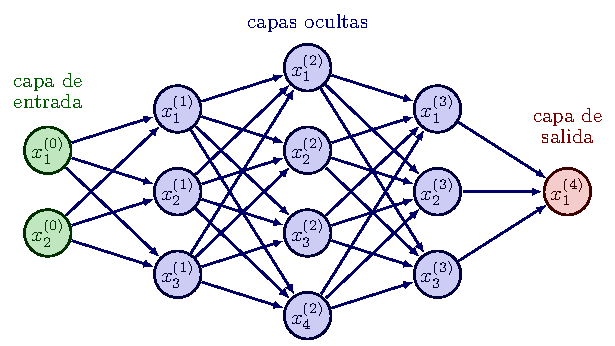
\includegraphics[width=0.5\textwidth]{img/neural_network/neural_network_feed_forward.pdf}
		\caption{Representación de una FFNN con cuatro capas. Elaboración propia.}
		\label{fig:ejemplo-red-neuronal}
	\end{figure}

	En este caso, la red neuronal se encuentra compuesta por cinco capas: una de entrada con $d_0 = 2$, tres ocultas con $d_1 = 3$, $d_2 = 4$, $d_3 = 3$, y una de salida con $d_4 = 1$. Cada uno de los nodos $x_i^{(\ell)}$ corresponde a la $i$-ésima \textit{neurona} de la capa $\ell$. Es este el motivo de porqué a $d_\ell$ se les refiere como el número de neuronas de la capa $\ell$. Además, se puede notar que, sin contar la capa de entrada, la red neural tiene una profundidad de $L = 4$ capas, de ahí que se le llame profundidad de la red.

	En este caso, la función $g^{(\ell)}_{\vth_\ell}$ es representada a través de los arcos que conectan las neuronas de la capa $\ell-1$ con las neuronas de la capa $\ell$. Por otro lado, las funciones de activación $\sigma^{(\ell)}$ se encuentran implícitamente utilizadas al definir recursivamente los vectores de neuronas $x^{(\ell)} \in \R^{d_\ell}$ de la siguiente manera:
	\begin{equation}
		x^{(\ell)} =
		\begin{cases}
			\vx,                                                         & \text{si } \ell = 0,           \\
			\sigma^{(\ell)} \circ g^{(\ell)}_{\vth_\ell} (x^{(\ell-1)}), & \text{en cualquier otro caso.}
		\end{cases}
		\quad \forall \ell = 0, \ldots, L.
	\end{equation}
	Es evidente concluir que la salida de la red neuronal es $f_{\vth}(\vx) = x^{(L)}$.
\end{example}

La razón por la que las redes neuronales han tenido tanto éxito en los últimos años se debe a que estas son capaces de aprender funciones muy complejas, siempre y cuando estas posean el número de parámetros suficientes y la cantidad de datos necesario.
Este hecho es demostrado por George Cybenko en 1989 en su Teorema de Aproximación Universal (UAT por sus siglas en inglés) \cite{cybenko1989approximation}.

A pesar de que la primera versión del UAT fue propuesta por Cybenko en 1989, el teorema fue popularizado por Kurt Hornik en 1991 \cite{hornik1991approximation}, debido a que en el teorema de Cybenko utiliza una función de activación sigmoide, mientras que en la versión de Hornik lo extiende a una función de activación continua. Por este motivo, es que a continuación se presenta la versión de Hornik del UAT.
\begin{theorem}[Teorema de Aproximación Universal \cite{hornik1991approximation}]\label{thm:universal-approximation-theorem}
	Sea $\sigma \in \ContSpace[\R, \R]$ una función de activación continua.
	Sean $d_0, d_2 \in \N$, números naturales, $K \subseteq \R^{d_0}$ un conjunto compacto y $f \in \ContSpace[K, \R^{d_2}]$ la función a aproximar.
	Entonces, $\sigma$ no es polinomial sí y sólo sí para cada $\epsilon > 0$, existe $d_1\in\N$, $\vW \in \R^{d_1 \times d_0}$, $b \in \R^{d_1}$ y $C \in \R^{d_2 \times d_1}$ tal que:
	\begin{equation}
		\sup_{\vx \in K} \left\| f(\vx) - C \cdot \sigma(\vW \cdot \vx + b) \right\| < \epsilon.
	\end{equation}
\end{theorem}

\begin{remark}
	El Teorema~\ref{thm:universal-approximation-theorem} establece que una red neuronal de una única capa oculta con una función de activación no polinomial (como por ejemplo, una sigmoide) es capaz de aproximar cualquier función continua en un conjunto compacto $K$ con un error arbitrariamente pequeño. Sin embargo, este teorema no establece cuántas neuronas en la capa oculta son necesarias para aproximar dicha función, ni tampoco establece cómo se deben de escoger los parámetros de la red neuronal.
\end{remark}

Con el paso de los años, se han propuesto diversas versiones del UAT. Sin embargo, el Teorema~\ref{thm:universal-approximation-theorem} ya ilustra de manera efectiva por qué las redes neuronales son tan efectivas en la aproximación de funciones.

Este capítulo concluye destacando la existencia de múltiples variantes de las redes neuronales, entre las que se incluyen las Redes Neuronales Convolucionales (CNN por sus siglas en inglés) y las Redes Neuronales Recurrentes (RNN por sus siglas en inglés). Estas variantes han ganado popularidad en los campos de la visión computacional y del procesamiento de lenguaje natural, respectivamente. Específicamente, en el presente trabajo se emplean las Redes Neuronales Convolucionales.



\section{Redes Generativas Adversarias}\label{sec:redes-generativas-adversarias-GAN}  % MARK: Redes Generativas Adversarias

Comencemos esta sección imaginando la siguiente situación\footnote{Este ejemplo es una adaptación y fue inspirado de \cite[min. 4:32]{santana2017creando}}:
\begin{quotation}
	\textit{Supongamos que hay un ladrón que desea engañar a un policía entregándole un billete falso. El ladrón, que es un inexperto, le entrega una servilleta, con una cara dibujada en ella, y que en el otro lado de la servilleta tiene escrito: ``\emph{esto vale un millón de dólares}''. El policía, que ha sido entrenado en la detección de billetes falsos, revisa el billete para comprobar que, efectivamente, es un billete falso.}

	\textit{Sin embargo, en vez de enviar a la cárcel al ladrón, lo que hace es decirle al ladrón cuales fueron sus fallos, y de qué manera puede este mejorar en sus falsificaciones. Por su parte, el policía también se entrena más y más en la detección de billetes falsos, pues puede que en algún momento, el ladrón se vuelva tan bueno en la elaboración de billetes falsos, que llegue a engañar al policía con uno de sus billetes.}
\end{quotation}

\begin{figure}[htbp]
	\centering
	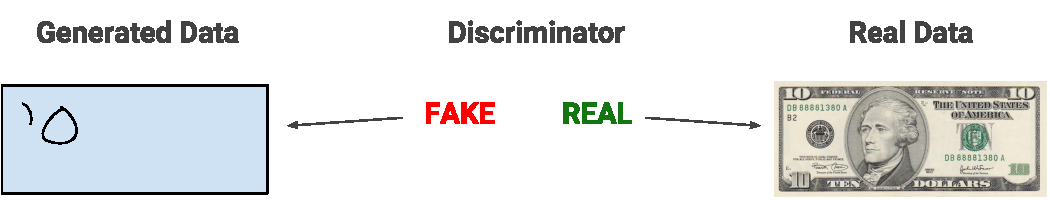
\includegraphics[width=0.7\textwidth]{img/gan/bad_gan.pdf}\vspace{0.6cm}
	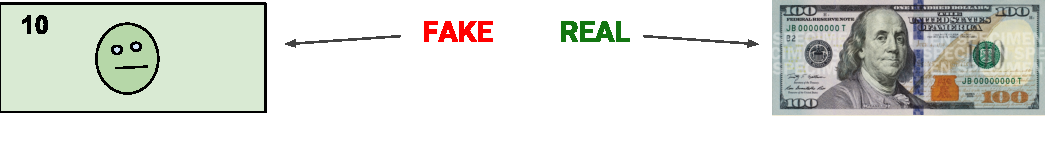
\includegraphics[width=0.7\textwidth]{img/gan/ok_gan.pdf}
	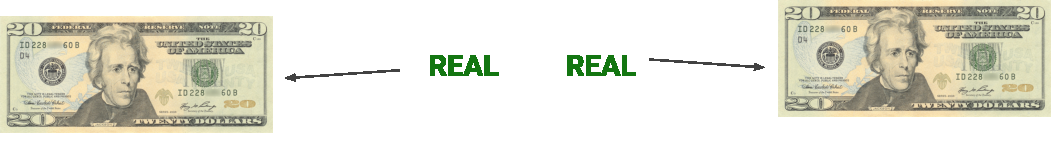
\includegraphics[width=0.7\textwidth]{img/gan/good_gan.pdf}
	\caption{Visualización gráfica de la analogía del ladrón y el policía en las GAN. Imagen obtenida de \cite{googlegan}.}
	\label{fig:gan-analogy}
\end{figure}

El marco de las Redes Generativas Adversarias (GAN), introducido en el trabajo de Goodfellow et al. \cite{goodfellow2014generative}, es en esencia, la analogía del ladrón y el policía.
La GAN define un juego donde el objetivo de la \emph{generadora} (el ladrón) es la de generar muestras que parezcan reales, mientras que el objetivo de la \emph{discriminadora} (el policía) es el de clasificar las muestras como verdaderas o falsas.
En este caso, la generadora se entrena para engañar a la discriminadora, y la discriminadora se entrena para detectar la falsedad de las muestras generadas.

En la siguiente subsección define formalmente una GAN, presenta los teoremas de convergencia de la GAN, y se describe el algoritmo de entrenamiento de una GAN. En las subsecciones posteriores a esta se presentan las variantes de las GAN, como las WGAN, WGAN-GP y WGAN-LP, elementos necesarios para una de las partes de esta tesis.

\subsection{GAN}\label{ssec:GAN}
% MARK: GAN

En este trabajo de tesis se plantea una definición formal de una GAN, en el contexto no paramétrico, y utilizando medidas de probabilidades generales. Este enfoque es diferente al que se plantea en el \textit{paper} original \cite{goodfellow2014generative}, donde se utiliza una formulación no paramétrica, pero asumiendo que las medidas de probabilidad poseen densidad. Por tanto, se utiliza la formulación presentada en \cite{wikipediagan}, la cuál se basa en medidas de probabilidad generales, aunque se reescriben los teoremas y demostraciones para garantizar su formalidad. Estos se pueden encontrar en el Anexo~\ref{chap:demostraciones-adicionales-teos-gan}.

Desde el punto de vista de la teoría de juegos, la GAN se define como un juego de dos jugadores: una \textit{generadora} $\Prob_G$, donde su conjunto de estrategias es $\ProbSpace[\cX]$ (con $\cX$ el \textit{conjunto de referencia}, e.g. $\cX=[0, 1]^{n_1\times n_2}$ para un conjunto de imágenes), y una \textit{discriminadora} $\Prob_D(\dd y \mid x)$, donde su conjunto de estrategias es el conjunto de kernels Markovianos. Con esto, la GAN es un juego de suma cero con la siguiente función valor objetivo:
\begin{equation}
	\label{eq:gan-objective}
	V(\Prob_G, \Prob_D)
	= \Exp_{X\sim\Prob_G}{\Exp_{Y \sim \Prob_D(\dd y \mid X)} \left[ \ln Y \right]}
	+ \Exp_{\tilde X\sim\Prob_G}{\Exp_{Y \sim \Prob_D(\dd y \mid \tilde X)} \left[ \ln (1 - Y) \right]},
\end{equation}
donde la generadora busca minimizar la función valor, mientras que la discriminadora busca maximizar esta cantidad.

El objetivo final de la generadora es el de encontrar una distribución $\Prob_G$ tal que se aproxime a una distribución de referencia $\Prob_X \in \ProbSpace[\cX]$ (del cuál se tiene acceso a través de una medida empírica $\hat \Prob_X = \frac{1}{N} \sum_{i=1}^{N} \delta_{x_i}$). Por el otro lado, el objetivo de la discriminadora es el de clasificar las muestras verdaderas y falsas, asignándole valores cercano a 1 y 0 respectivamente.

El siguiente teorema nos habla acerca de la naturaleza del discriminador óptimo:

\begin{theorem}[El discriminador óptimo calcula la divergencia de JS]
	\label{thm:gan-optimal-discriminator}
	Para cualquier estrategia de generador $\Prob_G$ fijo, existe un único discriminador óptimo $\Prob_D^\ast$ que maximiza la función objetivo \eqref{eq:gan-objective}, el cuál toma una forma determinista por medio de $\Prob_D^\ast(\dd y \mid x) = \delta_{D^\ast(x)}(\dd y)$, donde $D^\ast(x) = \dv{\Prob_X}{(\Prob_G+\Prob_X)}$. En tal caso, la función valor toma la siguiente forma:
	\begin{equation}
		V(\Prob_G, \Prob_D^\ast) = \JS{\Prob_X}{\Prob_G} - 2 \ln 2.
	\end{equation}
\end{theorem}

\begin{proof}
	La demostración de este teorema se encuentra en el Anexo~\ref{chap:demostraciones-adicionales-teos-gan}.
\end{proof}

Este teorema nos dice que el discriminador óptimo es aquel que calcula la divergencia de Jensen-Shannon entre la distribución de referencia $\Prob_X$ y la distribución generada $\Prob_G$, salvo una constante. Además, nos dice que el discriminador toma una forma determinista, de forma que bastaría con buscar una función (como por ejemplo, una red neuronal) $D\colon\cX\to [0, 1]$ tal que la aproxime.

Dado que para cada generador $\Prob_G$ existe un único discriminador óptimo $\Prob_D^\ast$, entonces tiene sentido definir la siguiente función:
\begin{equation}
	C(\Prob_G) \eqdef V(\Prob_G, \Prob_D^\ast) = \JS{\Prob_X}{\Prob_G} - 2 \ln 2.
\end{equation}
El siguiente teorema nos dice que existe un único generador óptimo $\Prob_G^\ast$ que minimiza la función $C(\Prob_G)$, y que este corresponde a la distribución de referencia $\Prob_X$:

\begin{theorem}\label{thm:gan-optimal-generator}
	El mínimo global de la función $C(\Prob_G)$ se alcanza en $\Prob_G^\ast = \Prob_X$, y el valor mínimo es $C(\Prob_X) = - \ln 4$.
\end{theorem}

\begin{proof}
	La demostración de este teorema se encuentra en el Anexo~\ref{chap:demostraciones-adicionales-teos-gan}.
\end{proof}

En la práctica, la forma de implementar la generadora es a través de un \emph{modelo generativo de espacio latente}. Esto es,
\begin{equation}\label{eq:generative-model}
	\Prob_G (\dd x) \eqdef \int_\cZ \Prob_G(\dd x \mid z) \; \Prob_Z \left( \dd z\right),
\end{equation}
donde $\cZ$ es el espacio de las variables latentes, y $\Prob_Z \in \ProbSpace[\cZ] $ es la distribución del espacio latente (típicamente se utiliza la distribución Gaussiana o Uniforme).

Por simplicidad, el modelo generativo $\Prob_G (\dd x \mid z)$ se mapea de forma determinista a través de $\Prob_G (\dd x \mid z) = \delta_{G(z)}(\dd x)$, utilizando una función $G\colon \cZ \to \cX$, la cuál se estima a través de una red neuronal $G_\theta$. Por otro lado, el Teorema~\ref{thm:gan-optimal-discriminator} dice que, en el óptimo, el discriminador toma una forma determinista, de forma que basta con buscar una función $D\colon\cX\to [0, 1]$, la cual también se estima a través de una red neuronal $D_\varphi$.

\FM{Agregar una explicación de las funciones de pérdida para este caso, explicar qué cosas buscan minimizar/maximizar y describir el algoritmo de entrenamiento.}

Con el fin de definir un algoritmo para entrenar una GAN, se definen las siguientes funciones de pérdida para la generadora y la discriminadora:
\begin{align}
	\cL_{\mathrm{disc}} & = -\frac{1}{N}\sum_{i=1}^{N} \Big[ \ln D_\varphi(x_i) + \ln \qty\big(1 - D_\varphi(G_\theta(z_i))) \Big], \\
	\cL_{\mathrm{gen}}  & = - \frac{1}{N}\sum_{i=1}^{N} \ln \qty\big(D_\varphi(G_\theta(z_i))),
\end{align}
donde $\{x_i\}_{i=1}^{N} \sim \Prob_X$ y $\{z_i\}_{i=1}^{N} \sim \Prob_Z$ son muestras del conjunto de entrenamiento y del espacio latente, respectivamente. La función de pérdida $\cL_{\mathrm{disc}}$ proviene de buscar maximizar la función objetivo \eqref{eq:gan-objective}, mientras que la función de pérdida $\cL_{\mathrm{gen}}$ se deriva de buscar minimizar la misma función objetivo.

De esta manera, el Algoritmo~\ref*{alg:GAN} describe la forma de estimar los parámetros $\theta$ y $\varphi$ de la generadora y la discriminadora, respectivamente. Usualmente, el flujo de este algoritmo se realiza en dos pasos: primero se actualiza la discriminadora $D_\varphi$ por $N_d$ iteraciones, y luego se actualiza la generadora $G_\theta$ por una iteración. Este proceso se repite hasta que los parámetros $\theta$ converjan.

\begin{algorithm}[H]
	\caption{Entrenamiento de una Red Generativa Adversaria}\label{alg:GAN}
	\begin{algorithmic}[1]
		\Require Tamaño del batch $N$ y número de iteraciones para el discriminador $N_d$.
		\State Inicializar los parámetros de la generadora $G_\theta$ y la discriminadora $D_\varphi$.
		\While{$\theta$ no ha convergido}
		\For{$t=1,\ldots,N_d$}
		\State Muestrear $\{x_i\}_{i=1}^{N} \sim \Prob_X$ desde el conjunto de entrenamiento.
		\State Muestrear $\{z_i\}_{i=1}^{N} \sim \Prob_Z$ desde el espacio latente.
		\State $\cL_{\mathrm{disc}} \gets -\frac{1}{N}\sum_{i=1}^{N} \Big[ \ln D_\varphi(x_i) + \ln \qty\big(1 - D_\varphi(G_\theta(z_i))) \Big]$
		\State Actualizar $D_\varphi$ por medio de descenso de gradiente en $\pdv{\varphi} \cL_{\mathrm{disc}}$.
		\EndFor
		\State Muestrear $\{z_i\}_{i=1}^{N} \sim \Prob_Z$ desde el espacio latente.
		\State $\cL_{\mathrm{gen}} \gets - \frac{1}{N}\sum_{i=1}^{N} \ln \qty\big(D_\varphi(G_\theta(z_i)))$
		\State Actualizar $G_\theta$ por medio de descenso de gradiente en $\pdv{\theta} \cL_{\mathrm{gen}}$.
		\EndWhile
	\end{algorithmic}
\end{algorithm}

\begin{remark}
	El Algoritmo~\ref{alg:GAN} empieza por determinar el óptimo de $\max_D V( \Prob_G , \Prob_D )$, el cuál proporciona una aproximación para la divergencia de Jensen-Shannon entre $\Prob_X$ y $\Prob_G$. Luego, actualiza la generadora $G$ para minimizar dicha divergencia. Con este procedimiento, la distribución $\Prob_G$ converge a la distribución de referencia $\Prob_X$ \textbf{utilizando la divergencia de Jensen-Shannon}.
\end{remark}

Es común que las arquitecturas de tipo GAN sean representadas como en la Figura~\ref{fig:gan-diagram}. En esta figura, se puede observar que la generadora $G$ toma una variable latente $z$ y la mapea a una muestra $\tilde x$, mientras que la discriminadora $D$ toma una muestra $x$ y la clasifica como verdadera o falsa.

\begin{figure}[H]
	\centering
	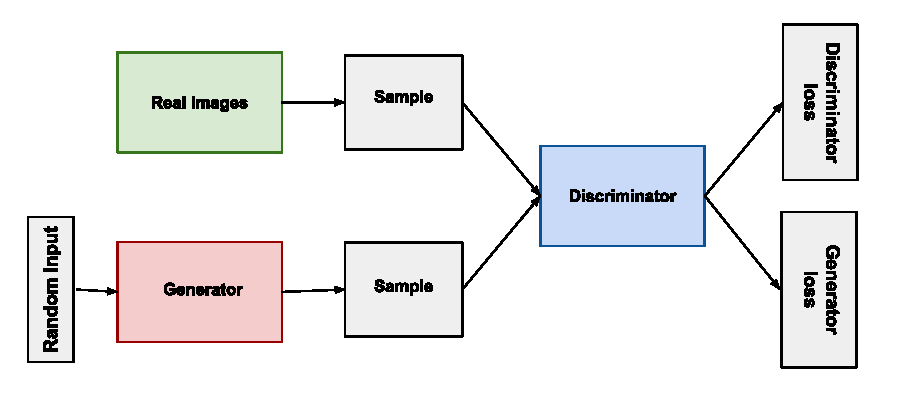
\includegraphics[width=0.75\textwidth]{img/gan/gan_diagram.pdf}
	\caption{Representación gráfica de la arquitectura de una GAN. Imagen obtenida de \cite{googlegan}.}
	\label{fig:gan-diagram}
\end{figure}


\FM[inline]{Si es que en el futuro se puede, modificar esta figura para que coincida más con la descripción}

% Teorema de la GAN: Convergencia en divergencia Jensen-Shannon

% Ejemplos?


\subsection{Wasserstein GAN}\label{ssec:wasserstein-gan}  % MARK: WGAN

La Wasserstein GAN (WGAN) \cite{arjovsky2017wasserstein} es una variante de las GANs que propone una nueva función de pérdida basada en la distancia de Wasserstein, en lugar de la divergencia de Jensen-Shannon. La principal ventaja de la WGAN es que es más estable y efectiva en la generación de datos, evitando problemas como el modo de colapso y el desvanecimiento del gradiente.

La función de pérdida se basa en el teorema de dualidad de Kantorovich-Rubinstein, el cuál se enuncia a continuación:
\begin{theorem}[Teorema de dualidad de Kantorovich-Rubinstein \cite{villani2009optimal}]\label{thm:dualidad-kantorovich-rubinstein}
	Sean $\Prob, \ProbQ \in \WassersteinSpace[1]{\cX}$ dos medidas de probabilidad en un espacio métrico $\cX$. Entonces, la distancia de Wasserstein entre $\Prob$ y $\ProbQ$ se puede expresar como:
	\begin{equation}\label{eq:dualidad-kantorovich-rubinstein}
		\Wasserstein[1]{\Prob}{\ProbQ} = \sup_{f \in \Lip[\cX]} \left\{ \Exp_{X\sim \Prob} [f(X)] - \Exp_{\tilde X \sim \ProbQ} [f(\tilde X)] \right\}.
	\end{equation}
\end{theorem}

Inspirados en este teorema, los autores de la WGAN \cite{arjovsky2017wasserstein} reemplazan el anterior juego de la GAN por el siguiente:
\begin{equation}\label{eq:wgan-game}
	(P_{\mathrm{WGAN}}) \quad \min_{G} \max_{f \in \Lip[\cX]} \Exp_{X\sim \Prob_X} [f(X)] - \Exp_{\tilde X \sim \Prob_G} [f(\tilde X)],
\end{equation}
donde la función $G$ es la \textit{generadora} y $f$ es la \textit{función crítica}. Se puede destacar que en este juego, el primer objetivo es obtener una estimación de la distancia de Wasserstein, para después utilizar esta estimación para minimizar la distancia entre la distribución real y la generada.

En la práctica, se utilizan las redes neuronales $G_\theta: \cZ \to \cX$ y $f_\omega: \cX \to \R$ para aproximar la generadora y la función crítica, respectivamente.
La generadora $G_\theta$ busca, como en el caso de la GAN, minimizar la distancia entre la distribución real y la generada, mientras que la función crítica $f_\omega$ busca maximizar la expresión en~\eqref{eq:dualidad-kantorovich-rubinstein}, con la restricción de que sea $1$-Lipschitz.

Este procedimiento define a la función de pérdida como
la diferencia entre la media de la función crítica evaluada en las muestras reales y generadas, lo que proporciona una estimación de la distancia de Wasserstein:
\begin{equation}\label{eq:wasserstein-estimation}
	\widehat W_N^{(1)} (
	\omega, \theta, x, z
	)
	\eqdef \frac{1}{N}\sum_{i=1}^{N} f_\omega(x_i) - \frac{1}{N}\sum_{i=1}^{N} f_\omega(G_\theta(z_i)),
\end{equation}
donde $x = (x_i)_{i=1}^{N} \sim \Prob_X$ y $z = (z_i)_{i=1}^{N} \sim \Prob_Z$ son muestras de las distribuciones reales y del espacio latente, respectivamente.

Más específicamente, las funciones de pérdida para la generadora y la función crítica son las siguientes:
\begin{align}
	\cL_{\mathrm{critic}}(\omega)
	 & = -\widehat W_N^{(1)} (
	\omega, \theta, x, z
	)
	= \frac{1}{N}\sum_{i=1}^{N} f_\omega(G_\theta(z_i)) - \frac{1}{N}\sum_{i=1}^{N} f_\omega(x_i),
	\\ \cL_{\mathrm{gen}}(\theta)
	 & = \widehat W_N^{(1)} (
	\omega, \theta, x, z
	)
	= -\frac{1}{N}\sum_{i=1}^{N} f_\omega(G_\theta(z_i)).
\end{align}
Destacando que, como la función de pérdida busca maximizar $\cL$, entonces este cambia su signo. Por otro lado, la función de pérdida de la generadora busca minimizar $\cL$, pero descarta los términos que no dependan de $\theta$.

Con el fin de asegurarse que la función crítica $f_\omega$ sea $1$-Lipschitz, en el trabajo original se proponía la restricción de que los pesos de la red fueran acotados. Esta restricción empeora el desempeño de la red, por lo que se han propuesto otras alternativas para garantizar que la red neuronal $f_\omega$ sea $1$-Lipschitz. Estas variaciones se revisarán en las siguientes subsecciones.

Paso seguido, la generadora utiliza la aproximación de la distancia de Wasserstein para minimizar la distancia entre la distribución real y la generada (recordando que esta se obtiene a través de un modelo generativo de espacio latente).

De este modo, el algoritmo de entrenamiento de la WGAN se resume en el Algoritmo~\ref{alg:WGAN}.

\begin{algorithm}[H]
	\caption{Entrenamiento de una Wasserstein GAN}\label{alg:WGAN}
	\begin{algorithmic}[1]
		\Require Tamaño del batch $N$, número de iteraciones para el discriminador $N_d$ y el parámetro de clipping $c$.
		\State Inicializar los parámetros de la generadora $G_\theta$ y la función crítica $f_\omega$.
		\While{$\theta$ no ha convergido}
		\For{$t=1,\ldots,N_d$}
		\State Muestrear $\{x_i\}_{i=1}^{N} \sim \Prob_X$ desde el conjunto de entrenamiento.
		\State Muestrear $\{z_i\}_{i=1}^{N} \sim \Prob_Z$ desde el espacio latente.
		\State $\cL_{\mathrm{critic}} \gets
			\frac{1}{N} \sum_{i=1}^{N} f_{\omega}(G_\theta(z_i)) - \frac{1}{N} \sum_{i=1}^{N} f_{\omega}(x_i)$ \Comment{$\cL_{\mathrm{critic}} = -\widehat W_N^{(1)}$}
		\State Actualizar $f_{\omega}$ por medio de descenso de gradiente en $\pdv{\omega} \cL_{\mathrm{critic}}$.
		\State $\omega \gets \text{clip}(\omega, -c, c)$
		\EndFor
		\State Muestrear $\{z_i\}_{i=1}^{N} \sim \Prob_Z$ desde el espacio latente.
		\State $\cL_{\mathrm{gen}} \gets - \frac{1}{N}\sum_{i=1}^{N} f_\omega(G_\theta(z_i))$ \Comment{
		$\cL_{\mathrm{gen}} = \widehat W_N^{(1)}$
		}
		\State Actualizar $G_\theta$ por medio de descenso de gradiente en $\pdv{\theta} \cL_{\mathrm{gen}}$.
		\EndWhile
	\end{algorithmic}
\end{algorithm}

\FM[inline]{Agregar la explicación de que ahora, gracias a que se utiliza la distancia de wasserstein, estas medidas terminan convergiendo débilmente a la distribución de referencia (lo que lo hace más fácil de converjer)}

\subsection{Wasserstein GAN con Gradiente Penalizado}\label{ssec:}  % MARK: Wasserstein GAN con Gradiente Penalizado
Los autores de la WGAN reconocen que la restricción de que los pesos de la red sean acotados no es la mejor forma de garantizar que la función crítica sea $1$-Lipschitz. Por ello, proponen una nueva forma de garantizar esta restricción, mediante la penalización de gradientes \cite{gulrajani2017improved}. Esta técnica es llamada Wasserstein GAN con Gradiente Penalizado (WGAN-GP).

La idea por detrás de esta técnica proviene del siguiente corolario:

\begin{corollary}[Corolario 1 de \cite{gulrajani2017improved}]\label{cor:gradiente-penalizado}
	Sea $f^\ast$ la función que minimiza el problema de optimización del Teorema de dualidad de Kantorovich-Rubinstein (ver la Ecuación~\eqref{eq:dualidad-kantorovich-rubinstein} del Teorema~\ref{thm:dualidad-kantorovich-rubinstein}). Entonces, la norma del gradiente de $f^\ast$ es $1$ en casi todo punto bajo las distribuciones $\Prob$ y $\ProbQ$. Es decir,
	\begin{equation}
		\Exp_{Y\sim\tau} \qty\Big[ \norm{\nabla f^\ast(Y)} ] = 1,
	\end{equation}
	donde $\tau$ es una distribución definida de forma que $u\sim\Uniform[0, 1]$, y $Y = uX + (1-u)\tilde X$ con $X\sim\Prob$ y $\tilde X\sim\ProbQ$.
\end{corollary}

La idea que hay por detrás de este corolario, es que basta penalizar la función de pérdida de la función crítica $f_\omega$ cuando su gradiente no sea $1$, para garantizar que esta sea $1$-Lipschitz. Es decir, que intercambian el problema de optimización de~\eqref{eq:wgan-game} por el siguiente:
\begin{equation}
	(P_{\mathrm{WGAN-GP}}) \quad \min_{G} \max_{f} \Exp_{X\sim \Prob_X} [f(X)] - \Exp_{\tilde X \sim \Prob_G} [f(\tilde X)] + \lambda \Exp_{Y\sim\tau} \qty\Big[ \qty(\norm{\nabla f(Y)} - 1)^2 ],
\end{equation}
donde $\lambda$ es un coeficiente de penalización y $\tau$ es una distribución definida como en el Corolario~\ref{cor:gradiente-penalizado}.

Además, como este es una penalización para la función crítica, entonces la función de pérdida de la generadora se mantiene igual a la de la WGAN. De esta forma, la función de pérdida para la función crítica se define de la siguiente manera:
\begin{align}
	p(\omega, x, \tilde x) & \eqdef \frac{1}{N} \sum_{i=1}^{N} \qty(
	\norm{\nabla f_\omega(u_i x_i + (1-u_i) \tilde x_i)} - 1
	)^2 ,
	\\ \cL_{\mathrm{critic}}(\omega) & \eqdef
	\frac{1}{N} \sum_{i=1}^{N} f_\omega(x_i) - \frac{1}{N} \sum_{i=1}^{N} f_\omega(\tilde x_i)
	+ \lambda p(\omega),
\end{align}
donde $u = (u_i)_{i=1}^{N} \sim \Uniform[0, 1]$, $x = (x_i)_{i=1}^{N} \sim \Prob_X$ y $\tilde x = (\tilde x_i)_{i=1}^{N} \sim \Prob_G$ son muestras de las distribuciones reales y generadas, respectivamente.


\begin{algorithm}[H]
	\caption{Penalización del Gradiente}\label{alg:gradient-penalty}
	\begin{algorithmic}[1]
		\Function{gradPenalty}{$\omega$, $x$, $\tilde x$}
		\State Muestrear $u = (u_i)_{i=1}^N \sim \Uniform[0, 1]$.
		\State $\hat x \gets (u_i x_i + (1-u_i) \tilde x_i)_{i=1}^{N}$
		\Comment{Interpolación lineal}
		\State \Return{ $ \frac{1}{N} \sum_{i=1}^{N} \qty(
				\norm{\nabla f_\omega(\hat x_i)} - 1
				)^2 $ }
		\Comment{$\Exp_{\hat x\sim\tau} \qty\Big[ \qty(\norm{\nabla f_\omega(\hat x)} - 1)^2 ]$}
		\EndFunction
	\end{algorithmic}
\end{algorithm}

Como este procedimiento se puede separar en dos pasos, se define un algoritmo para la penalización del gradiente, el cuál se presenta en el Algoritmo~\ref{alg:gradient-penalty}. Con este, se define el algoritmo de entrenamiento de la WGAN-GP en el Algoritmo~\ref{alg:WGAN-GP}.

\begin{algorithm}[H]
	\caption{Entrenamiento de una WGAN con Gradiente Penalizado}\label{alg:WGAN-GP}
	\begin{algorithmic}[1]
		\Require Tamaño del batch $N$, número de iteraciones para el discriminador $N_d$ y el parámetro de penalización $\lambda$.
		\State Inicializar los parámetros de la generadora $G_\theta$ y la función crítica $f_\omega$.
		\While{$\theta$ no ha convergido}
		\For{$t=1,\ldots,N_d$}
		\State Muestrear $\{x_i\}_{i=1}^{N} \sim \Prob_X$ desde el conjunto de entrenamiento.
		\State Muestrear $\{z_i\}_{i=1}^{N} \sim \Prob_Z$ desde el espacio latente.
		\State $\tilde x \gets (G_\theta(z_i))_{i=1}^{N}$.
		\State $\cL_{\mathrm{critic}} \gets
			\frac{1}{N} \sum_{i=1}^{N} f_{\omega}(\tilde x_i) - \frac{1}{N} \sum_{i=1}^{N} f_{\omega}(x_i) + \lambda \cdot \Call{gradPenalty}{\omega, x, \tilde x}$
		\State Actualizar $f_{\omega}$ por medio de descenso de gradiente en $\pdv{\omega} \cL_{\mathrm{critic}}$.
		\EndFor
		\State Muestrear $\{z_i\}_{i=1}^{N} \sim \Prob_Z$ desde el espacio latente.
		\State $\cL_{\mathrm{gen}} \gets - \frac{1}{N}\sum_{i=1}^{N} f_\omega(G_\theta(z_i))$
		\State Actualizar $G_\theta$ por medio de descenso de gradiente en $\pdv{\theta} \cL_{\mathrm{gen}}$.
		\EndWhile
	\end{algorithmic}
\end{algorithm}

\FM[inline]{Si queda tiempo, agregar la WGAN-LP para hablar de la WGAN-GGP}


\section{Auto-Encoders}\label{sec:auto-Encoders}  % MARK: Auto-Encoders

Junto con las GANs, otro tipo de arquitectura que ha sido muy popular en la comunidad del aprendizaje profundo son los Auto-Encoders (AE). Los AE son una arquitectura de redes neuronales que se utiliza para aprender una codificación eficiente de datos no etiquetados. En otras palabras, aprende a ``comprimir la información'' del conjunto de datos.

\subsection{AE}\label{ssec:AE}  % MARK: - AE

Al igual que en la sección anterior, se presenta una definición formal de un AE en el contexto no paramétrico, y utilizando medidas de probabilidad generales. En este caso, esta sección se basa en \cite{tolstikhin2017wasserstein}, aunque ha sido modificado en el contexto de los AE ``vainilla'' (y no en su versión Wasserstein, como se presenta en la referencia).

Un AE se compone de dos partes: un codificador (en inglés, \textit{encoder}) y un decodificador (en inglés, \textit{decoder}).
Un \textit{codificador} $ \ProbQ(\dz \mid x)$ corresponde a un kernel de transición tal que a cada $x \in \cX$ le asigna una distribución en el espacio latente $ \ProbSpace[\cZ] $.
Por el otro lado, un \textit{decodificador} $\Prob_G(\dx \mid z)$ corresponde a un kernel de transición tal que a cada $z \in \cZ$ le asigna una distribución en el espacio de referencia $\ProbSpace[\cX]$.
En este trabajo, se asume que el decodificador es determinista, es decir, que $\Prob_G(\dx \mid z) = \delta_{G(z)}(\dx)$, donde $G\colon \cZ \to \cX$ es una función.

En el objetivo de aprender una codificación eficiente, el AE busca minimizar el error de reconstrucción, denotado como $c(x, \tilde x)$. Este proceso se lleva a cabo de la siguiente manera: primero, se obtiene una muestra $x\sim \Prob_X$, luego se adquiere una representación latente mediante $\tilde z \sim \ProbQ(\dz \mid x)$ y finalmente se logra la reconstrucción a través de $\tilde x \sim \Prob_G(\dx \mid \tilde z)$. En este contexto, la función objetivo que el AE busca minimizar es:
\begin{equation}\label{eq:ae-obj-func}
	V(\ProbQ, \Prob_G) = \Exp_{X \sim \Prob_X} \Exp_{\tilde Z \sim \ProbQ(\dz \mid X)} \qty\big[ c(X, G(\tilde Z)) ].
\end{equation}

Cabe mencionar que en el caso en que el codificador también sea determinista, es decir, que $\ProbQ(\dz \mid x) = \delta_{E(x)}(\dz)$ con $E\colon \cX \to \cZ$ una función, entonces la variable aleatoria
$\Exp_{\tilde Z \sim \ProbQ(\dz \mid X)} \qty\big[ c(X, G(\tilde Z)) ]$ se reduce a simplemente a $c(X, G(E(X)))$. En este caso, la función objetivo se reduce a:
\begin{equation}\label{eq:ae-obj-func-deterministic}
	V(\ProbQ, \Prob_G) = \Exp_{X \sim \Prob_X} \qty\big[ c(X, G(E(X))) ].
\end{equation}

En la práctica, se puede asumir que el codificador se estima por medio de una red neuronal $\ProbQ_\varphi \left( \dd z \mid x \right)$, el cuál puede ser determinista o estocástica. Por otro lado, el decodificador $\Prob_G$ se puede aproximar por medio de una red neuronal $G_\theta$ de forma tal que $\Prob_G(\dd x \mid z) = \delta_{G_\theta(z)}(\dd x)$.
En este caso, la función de pérdida del AE se puede estimar de la siguiente manera:
\begin{equation}
	\cL_{\mathrm{AE}} = \frac{1}{N}\sum_{i=1}^{N} c(x_i, G_\theta(\tilde z_i)),
\end{equation}
donde $\{x_i\}_{i=1}^{N} \sim \Prob_X$ son muestras del conjunto de entrenamiento y $\{\tilde z_i\}_{i=1}^{N} \sim \ProbQ_\varphi \left( \dd z \mid x_i \right)$ son propagaciones hacia adelante de las muestras $x_i$ a través de la red neuronal $\ProbQ_\varphi$.

Dado lo anterior, el Algoritmo~\ref{alg:AE} describe la forma de estimar los parámetros $\varphi$ y $\theta$ del codificador y decodificador, respectivamente. Usualmente, el flujo de este algoritmo se realiza de forma iterativa hasta que los parámetros $\varphi$ y $\theta$ converjan.

\begin{algorithm}[H]
	\caption{Entrenamiento de un Auto-Encoder}\label{alg:AE}
	\begin{algorithmic}[1]
		\Require Tamaño del batch $N$.
		\State Inicializar los parámetros del codificador $\ProbQ_\varphi$ y del decodificador $G_\theta$.
		\While{$\varphi$ y $\theta$ no han convergido}
		\State Muestrear $\{x_i\}_{i=1}^{N} \sim \Prob_X$ desde el conjunto de entrenamiento.
		\State Muestrear $\tilde z_i \sim \ProbQ_\varphi \left( \dd z \mid x_i \right)$ para $i=1,\ldots,N$.
		\State $\cL_{\mathrm{AE}}\gets \frac{1}{N}\sum_{i=1}^{N} c(x_i, G_\theta(\tilde z_i))$.
		\State Actualizar $\ProbQ_\varphi$ y $G_\theta$ por medio de descenso de gradiente en $\pdv{\varphi} \cL_{\mathrm{AE}}$ y $\pdv{\theta} \cL_{\mathrm{AE}}$.
		\EndWhile
	\end{algorithmic}

\end{algorithm}


\subsection{Wasserstein AE}\label{ssec:WAE}  % MARK: WAE

Al igual que en el caso de la GAN, se puede definir una versión del AE que minimiza la distancia de Wasserstein entre la distribución real y la generada. En este caso, el Wasserstein AE (WAE) \cite{tolstikhin2017wasserstein} busca minimizar la distancia de Wasserstein entre la distribución real y la generada, en lugar de minimizar el error de reconstrucción. Esto lo logra utilizando el Teorema

\begin{theorem}[Teorema Fundamental del WAE \cite{tolstikhin2017wasserstein}]
	Sea $\Prob_X\in \ProbSpace$ cualquiera y  $\Prob_G\in \ProbSpace$ un modelo generativo definido como en la Ecuación~\eqref{eq:generative-model}, donde $\Prob_G(\dd x \mid Z) = \delta_{G(Z)}(\dd x)$ es determinista para cualquier función $G:\cZ \to \cX$. Entonces, se cumple lo siguiente:
	\begin{equation}
		\inf_{\pi\in\Cpl(\Prob_X, \Prob_G)} \Exp_{(X, Y)\sim\pi} \qty\big[ c(X, Y) ] = \inf_{\ProbQ \colon \ProbQ_Z = \Prob_Z} \Exp_{X\sim\Prob_X} \Exp_{\tilde Z\sim\ProbQ(\dd z \mid X)} \qty\big[ c(X, G(\tilde Z)) ],
	\end{equation}
	donde $\ProbQ_Z(\dd z) = \Exp_{X\sim \Prob_X} \qty[\ProbQ(\dd z \mid X)]$ corresponde a la marginal de $\ProbQ$ en el espacio latente.
\end{theorem}

Este teorema establece que, para cualquier función de pérdida $c$, la distancia de Wasserstein entre la distribución real y la generada se puede calcular de forma similar a un AE, utilizando un codificador $\ProbQ$ y un decodificador $G$. Es más, si es que se compara con la Ecuación~\eqref{eq:ae-obj-func}, se puede notar que son similares, pero con la diferencia de que en este caso, existe la restricción de que $\ProbQ_Z = \Prob_Z$.

Por tanto, el objetivo del WAE es \textbf{minimizar el error de reconstrucción, con la restricción de que la marginal del codificador sea igual a la distribución del espacio latente}. Con esto en mente, el problema de optimización del WAE corresponde a:
\begin{equation}
	(P_{\mathrm{WAE}}) \quad \min_{G} \min_{\ProbQ\colon \ProbQ_Z = \Prob_Z} \Exp_{X\sim\Prob_X} \Exp_{\tilde Z\sim\ProbQ(\dd z \mid X)} \qty\big[ c(X, G(\tilde Z)) ].
\end{equation}

Como se tiene una restricción de igualdad, se puede penalizar el problema anterior a través de alguna divergencia entre las distribuciones $\ProbQ_Z$ y $\Prob_Z$. En el trabajo original, se propone utilizar la discrepancia promedio máxima (MMD) \cite{gretton2006kernel} como divergencia. Este se define como:
\begin{equation}
	\MMDOp_k(\Prob_Z, \ProbQ_Z) = \Big\|
	\Exp_{Z\sim\Prob_Z} \qty\big[ k(Z, \cdot) ] - \Exp_{Z\sim\ProbQ_Z} \qty\big[ k(Z, \cdot) ]
	\Big\|_{\cH_k},
\end{equation}
donde $\cH_k$ es el RKHS asociado al kernel $k$.\FM{Creo que falta una cita aquí} De esta forma, el problema de optimización del WAE se puede reescribir como:
\begin{equation}
	(P_{\mathrm{WAE-MMD}}) \quad \min_{G} \min_{\ProbQ} \Exp_{X\sim\Prob_X} \Exp_{\tilde Z\sim\ProbQ(\dd z \mid X)} \qty\big[ c(X, G(\tilde Z)) ] + \lambda \cdot \MMDOp_{k}(\Prob_Z, \ProbQ_Z),
\end{equation}
para algún kernel $k$ y un coeficiente de penalización $\lambda > 0$.

La ventaja de utilizar la MMD como divergencia es que esta se comporta bien en el caso de que las distribuciones sean de alta dimensión, así como también para las distribuciones normales, además de poseer un estimador insesgado y consistente \cite{gretton2012kernel}:
\begin{equation}
	\widehat \MMDOp_k(z, \tilde z)
	= \frac{1}{n(n-1)} \sum_{i\neq j} k(z_i, z_j)
	+ \frac{1}{n(n-1)} \sum_{i\neq j} k(\tilde z_i, \tilde z_j)
	- \frac{2}{n^2} \sum_{i, j} k(z_i, \tilde z_j),
\end{equation}
donde $z = (z_i)_{i=1}^{n}$ y $\tilde z = (\tilde z_i)_{i=1}^{n}$ son muestras de las distribuciones $\Prob_Z$ y $\ProbQ_Z$, respectivamente.

\begin{algorithm}[H]
	\caption{Entrenamiento de una Wasserstein Auto-Encoder}\label{alg:WAE}
	\begin{algorithmic}[1]
		\Require Tamaño del batch $N$, kernel característico definido-positivo $k$ y el parámetro de penalización $\lambda$.
		\Function{MMD}{$z$, $\tilde z$}
		\State\Return{$\frac{1}{N(N-1)} \sum_{i\neq j} k(z_i, z_j) + \frac{1}{N(N-1)} \sum_{i\neq j} k(\tilde z_i, \tilde z_j) - \frac{2}{N^2} \sum_{i, j} k(z_i, \tilde z_j)$}
		\EndFunction
		\State Inicializar los parámetros del codificador $\ProbQ_\varphi$ y del decodificador $G_\theta$.
		\While{$\varphi$ y $\theta$ no han convergido}
		\State Muestrear $\{x_i\}_{i=1}^{N} \sim \Prob_X$ desde el conjunto de entrenamiento.
		\State Muestrear $\{z_i\}_{i=1}^{N} \sim \Prob_Z$ desde el espacio latente.
		\State Muestrear $\tilde z_i \sim \ProbQ_\varphi(\dd z \mid x_i)$ para $i=1\dots N$.
		\Comment{$\tilde z = \ProbQ_\varphi(x)$ si $\ProbQ_\varphi$ es determinista.}
		\State $\cL_{\mathrm{AE}} \gets \frac{1}{N}\sum_{i=1}^{N} c(x_i, G_\theta(\tilde z_i)) + \lambda \cdot \Call{MMD}{z, \tilde z}$.
		\State Actualizar $\ProbQ_\varphi$ y $G_\theta$ por medio de descenso de gradiente en $\pdv{\varphi} \cL_{\mathrm{AE}}$ y $\pdv{\theta} \cL_{\mathrm{AE}}$.
		\EndWhile
	\end{algorithmic}
\end{algorithm}


\section{Aplicación: Baricentros de Wasserstein Proyectados}\label{sec:app-bar-wass-Proyectados}  % MARK: - Section Aplicación: Baricentros de Wasserstein Proyectados

\RED[inline]{Hay que revisar esta sección!}
\RED[inline]{Aquí no me gusta como me refiero a cada rato a ``los autores'', hay que cambiarlo}

Una aplicación interesante de las GANs y AEs es que aprenden la variedad de imágenes de un conjunto de datos. Los autores de \cite{simon2020barycenters} proponen una forma de calcular baricentros de Wasserstein, utilizando una GAN y un AE como variedad de imágenes y proyector, respectivamente.

Aquel trabajo se enfoca en la interpolación de imágenes (también conocido como la morfización de imágenes), que se refiere a la transición visual de dos imágenes de entrada. Para que aquella transición sea visualmente atractiva, es deseable que cumpla con las siguientes propiedades: (\textit{i}) que sea suave, es decir, que no haya cambios bruscos en la transición; (\textit{ii}) que aplique los mínimos cambios necesarios en la imagen; y (\textit{iii}) que parezca ``realista'', evitando cambios no naturales en cada imagen de la transición.

Varias de estas propiedades se puede obtener a través de la interpolación de baricentros de Wasserstein, sin embargo, el resultado de esta interpolación puede no verse natural.
En base al trabajo \cite{zhu2016generative}, donde describe la manera en que una GAN aproxima una variedad de imágenes, y como se puede utilizar un AE para proyectar una imagen en esta variedad, los autores de \cite{simon2020barycenters} proponen utilizar una GAN y un AE para mantener la suavidad y realismo de la interpolación.

En la Figura~\ref{fig:interpolacion-wass-bar-gan} se puede observar un ejemplo de la interpolación de baricentros de Wasserstein, donde se puede notar que la interpolación es suave y realista.

\begin{figure}[H]
	\centering
	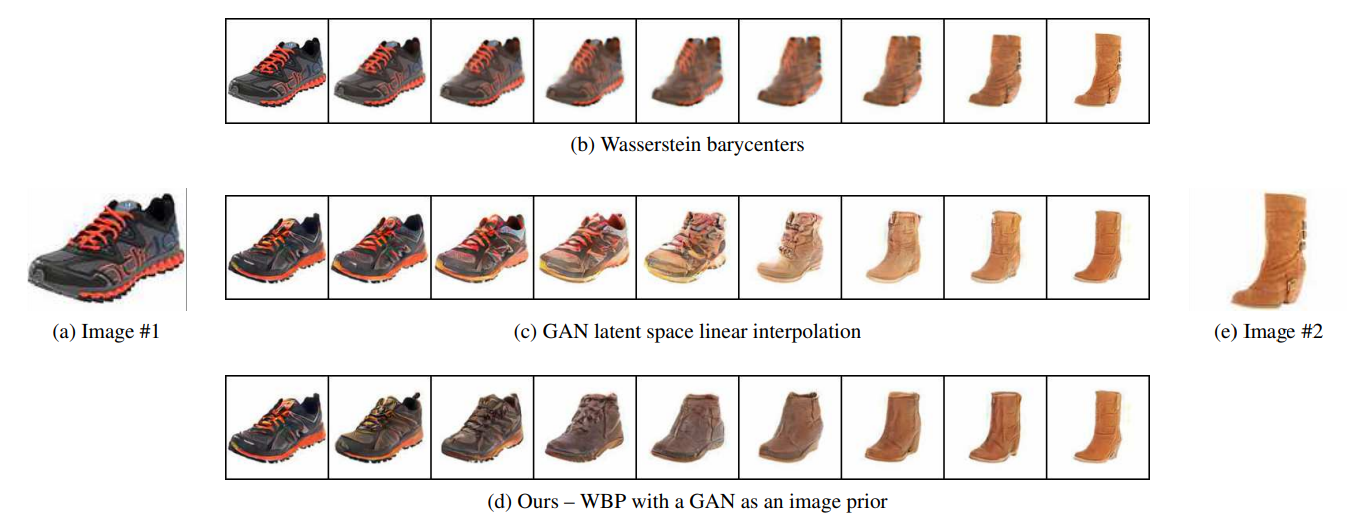
\includegraphics[width=\textwidth]{img/cbw/interpolacion-wass-bar-gan.png}
	\caption{
		Interpolación de una zapatilla deportiva a una bota utilizando 3 métodos. En la Figura~\ref{fig:interpolacion-wass-bar-gan} (b) las imágenes intermedias se ven borrosas y poco realistas. En la Figura~\ref{fig:interpolacion-wass-bar-gan} (c) la zapatilla a penas cambia y entonces inmediatamente cambia a una bota. En la Figura~\ref{fig:interpolacion-wass-bar-gan} (d) la interpolación es suave en la transición del color y de forma. Imagen obtenida de \cite{simon2020barycenters}.
	}
	\label{fig:interpolacion-wass-bar-gan}
\end{figure}


En \cite{simon2020barycenters}, se empieza asumiendo que el espacio $\cX$ en que se trabaja corresponde a una grilla de $n_1 \times n_2 = N$ píxeles, donde las medidas se encuentran definidas:
\begin{align*}
	\mu_0 = \sum_{i=1}^{N} p^{(0)}_i \delta_{x_i},
	\qquad \text{ y } \qquad
	\mu_1 = \sum_{i=1}^{N} p^{(1)}_i \delta_{x_i}.
\end{align*}
Por tanto, basta con considerar a los vectores $p^{(0)}$ y $p^{(1)}$ como vectores de probabilidad el Simplex $\Simplex[N] \eqdef \left\{ p \in [0, 1]^{N} \colon \sum_i p_i = 1 \right\}$.

De esta forma, los autores de \cite{simon2020barycenters} proponen el siguiente problema de optimización:
\begin{align*}
	(P_{\mathrm{CWB}}) \quad
	\min_{q \in \Simplex[N]} & \ \ (1-t) \Wasserstein[2]{\mu_0}{\nu}^2 + \Wasserstein[2]{\nu}{\mu_1}^2 \\
	\text{s.a.}              & \ \ \nu = \sum_{i=1}^{N} q_i \delta_{x_i} \in \bM,
\end{align*}
donde se puede notar que este problema es similar a la definición de una interpolación geodésica~\eqref{eq:interpolacion-geodesica}, pero con la diferencia de que se restringe a que el baricentro $\nu$ pertenezca a la variedad $\bM$. Por esta restricción, los autores llama a este problema como \textit{Baricentros de Wasserstein Restringidos} (CBW por sus siglas en inglés).

A partir del problema $(P_{\mathrm{CWB}})$, los autores imponen una restricción de igualdad en la variable $\nu$, de forma que $\tilde \nu = \nu$ con $\tilde \nu \in \bM$. De esta forma, se puede reescribir el problema $(P_{\mathrm{CWB}})$ utilizando la técnica del Lagrangiano Aumentado \cite[Sec. 2.3]{boyd2011distributed}:
\begin{align*}
	(P_{\mathrm{CWB}}^{\mathrm{AL}}) \quad
	\min_{q\in\Simplex[N],\tilde q,u} & \ \ (1-t) \Wasserstein[2]{\mu_0}{\nu}^2 + \Wasserstein[2]{\nu}{\mu_1}^2
	+ \frac{\rho}{2} \| \tilde q - q + u \|_2^2                                                                 \\
	\text{s.a.}                       & \ \ \tilde \nu = \sum_{i=1}^{N} \tilde q_i \delta_{x_i} \in \bM,
\end{align*}

El problema $(P_{\mathrm{CWB}}^{\mathrm{AL}})$ se puede resolver usando el Método de los Multiplicadores de Dirección Alterna (ADMM) \cite[Cap. 3]{boyd2011distributed} el cuál se presenta a continuación:

\begin{algorithm}[H]
	\caption{Baricentros de Wasserstein Restringidos (CBW)}\label{alg:ADMM-CWB}
	\begin{algorithmic}[1]
		\Require Vectores de probabilidad $p^{(0)}, p^{(1)} \in \Simplex[N]$, suposición inicial $q^{(0)}$, parámetro $t$, parámetro de penalización $\rho$ y umbral $\epsilon$.
		\State Inicializar $u^{(0)} \gets 0$, $\tilde q^{(0)} \gets q^{(0)}$, $k \gets 0$
		\Repeat
		\State $q^{(k+1)} \gets \argmin_{q\in\Simplex[N]}  (1-t) \Wasserstein[2]{\mu_0}{\nu}^2 + t\Wasserstein[2]{\nu}{\mu_1}^2 + \frac{\rho}{2} \| \tilde q^{(k)} - q + u^{(k)} \|_2^2$
		\State $\tilde q^{(k+1)} \gets \argmin_{\tilde q \colon \tilde \nu \in \bM } \| \tilde q - q^{(k+1)} + u^{(k)} \|_2^2 $
		\State $u^{(k+1)} \gets u^{(k)} + \tilde q^{(k+1)} - q^{(k+1)}$
		\State $k \gets k + 1$
		\Until{$\| q^{(k)} - \tilde q^{(k)} \|<\epsilon$}
		\State\Return $q^{(k)}$
	\end{algorithmic}
\end{algorithm}

Al principio, en la línea 3 del Algoritmo~\ref{alg:ADMM-CWB}, se encuentra una solución de la versión regularizada del problema de la Ecuación~\eqref{eq:interpolacion-geodesica} (los autores siguen \cite{cuturi2016smoothed} para resolver este problema). En la línea 4, se proyecta la solución en la variedad $\bM$ y en la línea 5 se actualiza la variable dual $u$. Este proceso se repite hasta que se alcance la convergencia.

En la Figura~\ref{fig:latent-pixel-space} se ilustra la diferencia entre su método, comparado con los otros dos métodos.

\begin{figure}[H]
	\centering
	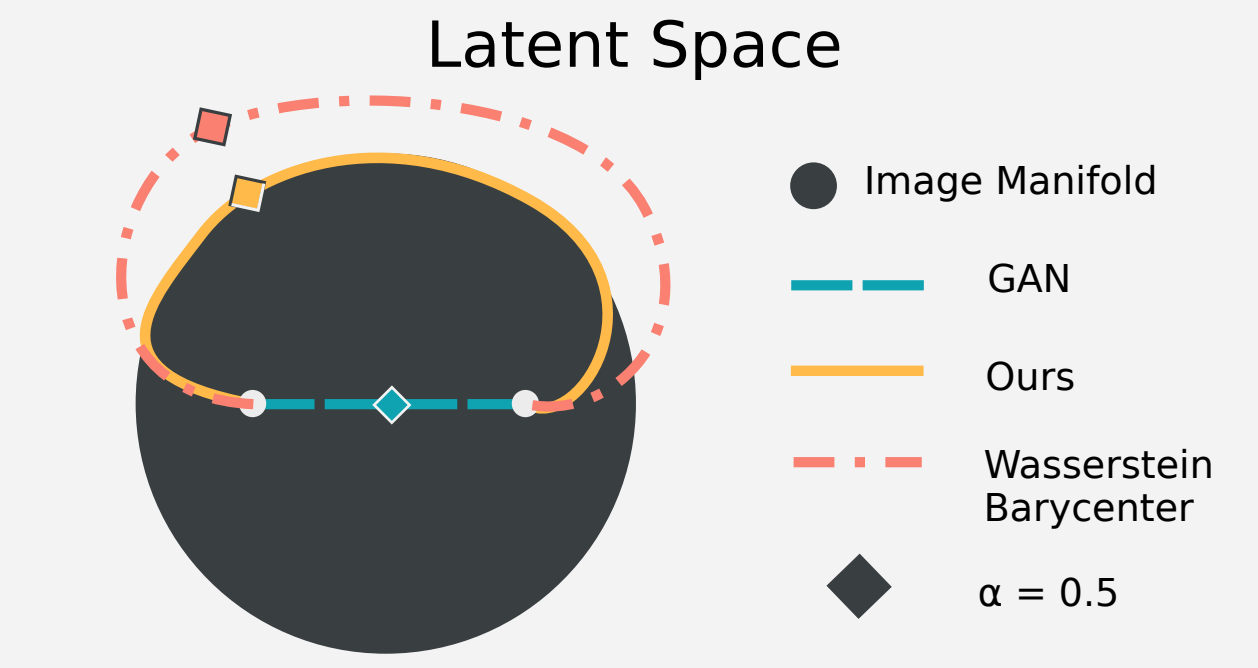
\includegraphics[width=0.48\textwidth]{img/cbw/latent-space.png}
	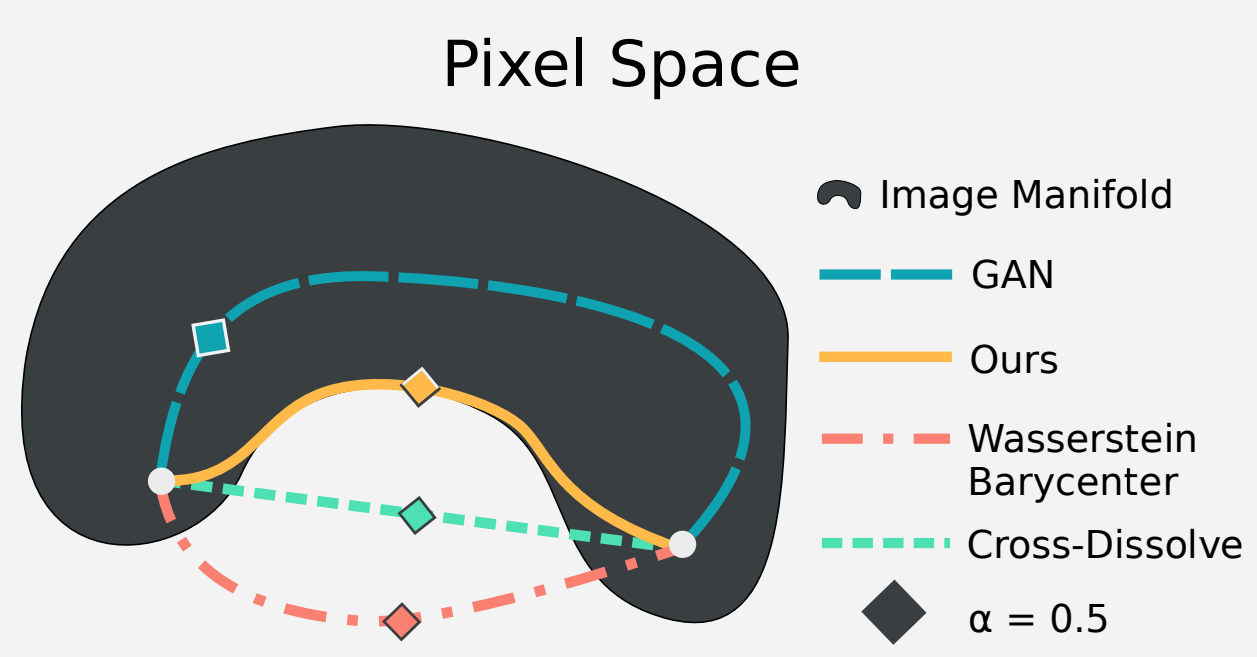
\includegraphics[width=0.48\textwidth]{img/cbw/pixel-space.png}
	\caption{
		Una ilustración del proceso de interpolación de una imagen, fijando $t = 0 \to 1$, usando varios métodos en el espacio de píxeles y en el espacio latente de una GAN entrenada.
		Imagen obtenida de \cite{simon2020barycenters}.
	}
	\label{fig:latent-pixel-space}
\end{figure}

\chapter{Modelos generativos basados en Wasserstein}
\label{chap:modelos-generativos-basados-en-Wasserstein}  % MARK: Modelos generativos basados en Wasserstein

En esta sección se revisan los modelos generativos basados en Wasserstein, como lo es la Wasserstein GAN (WGAN) \cite{arjovsky2017wasserstein} y el Wasserstein Auto-Encoder (WAE) \cite{tolstikhin2017wasserstein}. Estos modelos han sido propuestos como alternativas a las GANs y VAEs tradicionales, respectivamente, y han demostrado ser más estables y efectivos en la generación de datos.


\section{Wasserstein GAN}\label{sec:WGAN}  % MARK: Wasserstein GAN

La Wasserstein GAN (WGAN) \cite{arjovsky2017wasserstein} es una variante de las GANs que propone una nueva función de pérdida basada en la distancia de Wasserstein, en lugar de la divergencia de Jensen-Shannon utilizada en las GANs tradicionales. La principal ventaja de la WGAN es que es más estable y efectiva en la generación de datos, evitando problemas como el colapso del modo y el desvanecimiento del gradiente.

La función de pérdida se basa en el teorema de dualidad de Kantorovich-Rubinstein, el cuál se enuncia a continuación:
\begin{theorem}[Teorema de dualidad de Kantorovich-Rubinstein \cite{villani2009optimal}]\label{thm:dualidad-kantorovich-rubinstein}
    Sean $\Prob, \ProbQ \in \WassersteinSpace[1]{\cX}$ dos medidas de probabilidad en un espacio métrico $\cX$. Entonces, la distancia de Wasserstein entre $\Prob$ y $\ProbQ$ se puede expresar como:
    \begin{equation}\label{eq:dualidad-kantorovich-rubinstein}
        \Wasserstein[1]{\Prob}{\ProbQ} = \sup_{f \in \Lip[\cX]} \left\{ \Exp_{X\sim \Prob} [f(X)] - \Exp_{\tilde X \sim \ProbQ} [f(\tilde X)] \right\}.
    \end{equation}
\end{theorem}

Inspirados por el Teorema~\ref{thm:dualidad-kantorovich-rubinstein}, los autores de la WGAN \cite{arjovsky2017wasserstein} reemplazan el anterior juego de la GAN por el siguiente:
\begin{equation}
    \min_{G} \max_{f \in \Lip[\cX]} \Exp_{X\sim \Prob} [f(X)] - \Exp_{\tilde X \sim \ProbQ} [f(\tilde X)],
\end{equation}
donde la función $G$ es la \textit{generadora} y $f$ es la \textit{función crítica}. Se puede destacar que en este juego, el primer objetivo es obtener una estimación de la distancia de Wasserstein, para después utilizar esta estimación para minimizar la distancia entre la distribución real y la generada.

En la práctica, se utilizan las redes neuronales $G_\theta: \cZ \to \cX$ y $f_\omega: \cX \to \R$ para aproximar la generadora y la función crítica, respectivamente. La función crítica $f_\omega$ busca aproximar la función $f$ que maximiza la expresión en~\eqref{eq:dualidad-kantorovich-rubinstein}, con la restricción de que sea $1$-Lipschitz. Este procedimiento define una estimación de la distancia de Wasserstein de la siguiente manera:
\begin{equation}\label{eq:wasserstein-estimation}
    \widehat W_N^{(1)} (
    \omega
    ) \eqdef
    \frac{1}{N}\sum_{i=1}^{N} f_\omega(x_i) - \frac{1}{N}\sum_{i=1}^{N} f_\omega(\tilde x_i),
\end{equation}
donde $\{x_i\}_{i=1}^{N} \sim \Prob_X$ y $\{\tilde x_i\}_{i=1}^{N} \sim \Prob_G$ son muestras de las distribuciones reales y generadas, respectivamente.

% Inspirados por el Teorema~\ref{thm:dualidad-kantorovich-rubinstein}, los autores de la WGAN definen dos redes neuronales: una red generadora $G_\theta\colon\cZ\to\cX$ y la función crítica $f_\omega \colon \cX \to \R$, donde $\omega$ y $\theta$ son los parámetros de las redes. La función crítica $f_\omega$ busca aproximar la función $f$ que maximiza la expresión en~\eqref{eq:dualidad-kantorovich-rubinstein}, con la restricción de que sea $1$-Lipschitz. Este procedimiento define una estimación de la distancia de Wasserstein de la siguiente manera:
% \begin{equation}\label{eq:wasserstein-estimation}
%     \widehat W_N^{(1)} (
%     \omega
%     ) \eqdef
%     \frac{1}{N}\sum_{i=1}^{N} f_\omega(x_i) - \frac{1}{N}\sum_{i=1}^{N} f_\omega(\tilde x_i),
% \end{equation}
% donde $\{x_i\}_{i=1}^{N} \sim \Prob$ y $\{\tilde x_i\}_{i=1}^{N} \sim \ProbQ$ son muestras de las distribuciones reales y generadas, respectivamente.
% La función crítica $f_\omega$ se actualiza por medio de descenso de gradiente en $\pdv{\omega} \widehat W_\omega^{(1)}$.

Sin embargo, con el fin de asegurarse que la función crítica $f_\omega$ sea $1$-Lipschitz, en el trabajo original se proponía la restricción de que los pesos de la red fueran acotados. Esta restricción empeora el desempeño de la red, por lo que se han propuesto otras alternativas para garantizar que la red neuronal $f_\omega$ sea $1$-Lipschitz.

Paso seguido, la generadora utiliza la aproximación de la distancia de Wasserstein para minimizar la distancia entre la distribución real y la generada (recordando que esta se obtiene a través de un modelo generativo de espacio latente).

De este modo, el algoritmo de entrenamiento de la WGAN se resume en el Algoritmo~\ref{alg:WGAN}.

\begin{algorithm}[ht!]
    \caption{Entrenamiento de una Wasserstein GAN}\label{alg:WGAN}
    \begin{algorithmic}[1]
        \Require Tamaño del batch $N$, número de iteraciones para el discriminador $N_d$ y el parámetro de clipping $c$.
        % Penalization coefficients $\lambda_1, \lambda_2 > 0$, the number of critic iterations $n_{\text{critic}}$, the batch size $m$.
        \State Inicializar los parámetros de la generadora $G_\theta$ y la función crítica $f_\omega$.
        % Initialize the parameters of the encoder $Q_\phi$, \\generator/decoder $G_\theta$ and the critic function $f_\omega$.
        \While{$\theta$ no ha convergido}
        \For{$t=1,\ldots,N_d$}
        \State Muestrear $\{x_i\}_{i=1}^{N} \sim \Prob_X$ desde el conjunto de entrenamiento.
        \State Muestrear $\{z_i\}_{i=1}^{N} \sim \Prob_Z$ desde el espacio latente.
        % \State $\widehat W_N^{(1)} \gets - \left( \frac{1}{N}\sum_{i=1}^{N} f_{\omega}(x_i) - \frac{1}{N}\sum_{i=1}^{N} f_{\omega}(G_{\theta}(z_i)) \right)$
        \State $\cL_{\mathrm{critic}} \gets
            \frac{1}{N} \sum_{i=1}^{N} f_{\omega}(G_\theta(z_i)) - \frac{1}{N} \sum_{i=1}^{N} f_{\omega}(x_i)$ \Comment{$\cL_{\mathrm{critic}} = -\widehat W_N^{(1)}$}
        \State Actualizar $f_{\omega}$ por medio de descenso de gradiente en $\pdv{\omega} \cL_{\mathrm{critic}}$.
        \State $\omega \gets \text{clip}(\omega, -c, c)$
        % \State $\cL_{\mathrm{disc}} \gets -\frac{1}{N}\sum_{i=1}^{N} \Big[ \ln D_\varphi(x_i) + \ln \qty\big(1 - D_\varphi(G_\theta(z_i))) \Big]$
        % \State Actualizar $D_\varphi$ por medio de descenso de gradiente en $\pdv{\varphi} \cL_{\mathrm{disc}}$.
        % \State $\widehat W^{(1)}_{\omega}(\theta) \gets \frac{1}{m}\sum_{i=1}^{m} f_\omega(x_i) - \frac{1}{m}\sum_{i=1}^{m} f_\omega(G_\theta(z_i))$
        % \State $\cL_{\text{critic}} \gets -\widehat W^{(1)}_{\omega}(\theta) + \lambda_1 \cP(f_\omega)$
        % \State Update $f_\omega$ by descending $\pdv{\omega} \cL_{\text{critic}}$.
        \EndFor
        \State Muestrear $\{z_i\}_{i=1}^{N} \sim \Prob_Z$ desde el espacio latente.
        \State $\cL_{\mathrm{gen}} \gets - \frac{1}{N}\sum_{i=1}^{N} f_\omega(G_\theta(z_i))$ \Comment{
        $\cL_{\mathrm{gen}} = \widehat W_N^{(1)}$
        }
        % \State $\cL_{\mathrm{gen}} \gets - \frac{1}{N}\sum_{i=1}^{N} \ln \qty\big(D_\varphi(G_\theta(z_i)))$
        \State Actualizar $G_\theta$ por medio de descenso de gradiente en $\pdv{\theta} \cL_{\mathrm{gen}}$.
        % \State Update $G_\theta$ by descending $\pdv{\theta} \widehat W^{(1)}_{\omega}(\theta)$.
        % \State Sample $\tilde z_i \sim Q_\phi(dz | x_i)$ for $i=1,\ldots, m$.
        % \State $\widehat W^{(2)}_{\phi}(\theta) \gets \frac{1}{m}\sum_{i=1}^{m} |x_i - G_\theta(\tilde z_i)|$
        % \State $\cL_{\text{WAE}} \gets \widehat W^{(2)}_{\phi}(\theta) + \lambda_2 \cD(\{z_i\}_{i=1}^{m}, \{\tilde z_i\}_{i=1}^{m})$
        % \State Update $Q_\phi$ by descending $\pdv{\phi} \cL_{\text{WAE}}$.
        % \State Update $G_\theta$ by descending $\pdv{\theta} \widehat W^{(2)}_{\phi}(\theta)$.
        \EndWhile
    \end{algorithmic}
\end{algorithm}


\section{Variantes de la Wasserstein GAN}\label{sec:variantes-de-la-Wasserstein-GAN}  % MARK: Variantes de la Wasserstein GAN
\subsection{Wasserstein GAN con Gradiente Penalizado}\label{ssec:}  % MARK: Wasserstein GAN con Gradiente Penalizado
Los autores de la WGAN reconocen que la restricción de que los pesos de la red sean acotados no es la mejor forma de garantizar que la función crítica sea $1$-Lipschitz. Por ello, proponen una nueva forma de garantizar esta restricción, mediante la penalización de gradientes \cite{gulrajani2017improved}. Esta técnica es llamada Wasserstein GAN con Gradiente Penalizado (WGAN-GP).

La idea por detrás de esta técnica proviene del siguiente corolario:

\begin{corollary}[Corolario 1 de \cite{gulrajani2017improved}]\label{cor:gradiente-penalizado}
    Sea $f^\ast$ la función que minimiza la Ecuación~\eqref{eq:dualidad-kantorovich-rubinstein}. Entonces, la norma del gradiente de $f^\ast$ es $1$ en casi todo punto bajo las distribuciones $\Prob$ y $\ProbQ$.
\end{corollary}


\begin{algorithm}[ht!]
    \caption{Penalización del Gradiente}\label{alg:gradient-penalty}
    \begin{algorithmic}[1]
        \For{$t=1,\ldots,m$}
        \State Muestrear $\alpha \sim$.
        \EndFor
    \end{algorithmic}
\end{algorithm}

\begin{algorithm}[ht!]
    \caption{Entrenamiento de una WGAN-GP}\label{alg:WGAN-GP}
    \begin{algorithmic}[1]
        \Require Tamaño del batch $N$, número de iteraciones para el discriminador $N_d$ y el coeficiente de penalización $\lambda$.
        % Penalization coefficients $\lambda_1, \lambda_2 > 0$, the number of critic iterations $n_{\text{critic}}$, the batch size $m$.
        \State Inicializar los parámetros de la generadora $G_\theta$ y la función crítica $f_\omega$.
        % Initialize the parameters of the encoder $Q_\phi$, \\generator/decoder $G_\theta$ and the critic function $f_\omega$.
        \While{$\theta$ no ha convergido}
        \For{$t=1,\ldots,N_d$}
        \State Muestrear $\{x_i\}_{i=1}^{N} \sim \Prob_X$ desde el conjunto de entrenamiento.
        \State Muestrear $\{z_i\}_{i=1}^{N} \sim \Prob_Z$ desde el espacio latente.
        % \State $\widehat W_N^{(1)} \gets - \left( \frac{1}{N}\sum_{i=1}^{N} f_{\omega}(x_i) - \frac{1}{N}\sum_{i=1}^{N} f_{\omega}(G_{\theta}(z_i)) \right)$
        \State $\cL_{\mathrm{critic}} \gets
            \frac{1}{N} \sum_{i=1}^{N} f_{\omega}(G_\theta(z_i)) - \frac{1}{N} \sum_{i=1}^{N} f_{\omega}(x_i)$ \Comment{$\cL_{\mathrm{critic}} = -\widehat W_N^{(1)}$}
        \State Actualizar $f_{\omega}$ por medio de descenso de gradiente en $\pdv{\omega} \cL_{\mathrm{critic}}$.
        \State $\omega \gets \text{clip}(\omega, -c, c)$
        % \State $\cL_{\mathrm{disc}} \gets -\frac{1}{N}\sum_{i=1}^{N} \Big[ \ln D_\varphi(x_i) + \ln \qty\big(1 - D_\varphi(G_\theta(z_i))) \Big]$
        % \State Actualizar $D_\varphi$ por medio de descenso de gradiente en $\pdv{\varphi} \cL_{\mathrm{disc}}$.
        % \State $\widehat W^{(1)}_{\omega}(\theta) \gets \frac{1}{m}\sum_{i=1}^{m} f_\omega(x_i) - \frac{1}{m}\sum_{i=1}^{m} f_\omega(G_\theta(z_i))$
        % \State $\cL_{\text{critic}} \gets -\widehat W^{(1)}_{\omega}(\theta) + \lambda_1 \cP(f_\omega)$
        % \State Update $f_\omega$ by descending $\pdv{\omega} \cL_{\text{critic}}$.
        \EndFor
        \State Muestrear $\{z_i\}_{i=1}^{N} \sim \Prob_Z$ desde el espacio latente.
        \State $\cL_{\mathrm{gen}} \gets - \frac{1}{N}\sum_{i=1}^{N} f_\omega(G_\theta(z_i))$ \Comment{
        $\cL_{\mathrm{gen}} = \widehat W_N^{(1)}$
        }
        % \State $\cL_{\mathrm{gen}} \gets - \frac{1}{N}\sum_{i=1}^{N} \ln \qty\big(D_\varphi(G_\theta(z_i)))$
        \State Actualizar $G_\theta$ por medio de descenso de gradiente en $\pdv{\theta} \cL_{\mathrm{gen}}$.
        % \State Update $G_\theta$ by descending $\pdv{\theta} \widehat W^{(1)}_{\omega}(\theta)$.
        % \State Sample $\tilde z_i \sim Q_\phi(dz | x_i)$ for $i=1,\ldots, m$.
        % \State $\widehat W^{(2)}_{\phi}(\theta) \gets \frac{1}{m}\sum_{i=1}^{m} |x_i - G_\theta(\tilde z_i)|$
        % \State $\cL_{\text{WAE}} \gets \widehat W^{(2)}_{\phi}(\theta) + \lambda_2 \cD(\{z_i\}_{i=1}^{m}, \{\tilde z_i\}_{i=1}^{m})$
        % \State Update $Q_\phi$ by descending $\pdv{\phi} \cL_{\text{WAE}}$.
        % \State Update $G_\theta$ by descending $\pdv{\theta} \widehat W^{(2)}_{\phi}(\theta)$.
        \EndWhile
    \end{algorithmic}
\end{algorithm}
% \chapter{Segundo}

\lipsum[1-3]

\begin{definition}[ver \cite{KAR00}]
    Definición definitiva $$\frac{d}{dx}\int_a^xf(y)dy=f(x).$$
\end{definition}
% \chapter{Tercero}
\lipsum[50-60]
% \chapter{Conclusión}

\lipsum[130-132]
\begin{figure}
    \centering
    
\includegraphics[scale=.2]{img/logos/fcfm.pdf}
    \caption{Logo de la Facultad}
    \label{logofcfm}
\end{figure}

\lipsum[133-134]

\begin{table}
    \centering
    \caption{Tabla 1}
    \label{tabla:1}
    \begin{tabular}{|c|c|r|}
        \hline
        \textbf{Campo 1} & \textbf{Campo 2} & \textbf{Num} \\\hline
        Valor 1a         & Valor 2a         & 3            \\
        Valor 1b         & Valor 2b         & 3            \\
        \hline
    \end{tabular}

\end{table}

\lipsum[135]


% ver https://www.overleaf.com/learn/latex/Glossaries
% \input{lib/glosario.tex} % opcional

\nocite{*}
%%%%%%%% CITADO ANTIGUO %%%%%%%%%
% \bibliographystyle{unsrtnat}
% \bibliographystyle{IEEEtran}
% \bibliography{bibliografia.bib}

%%%%%%%% CITADO NUEVO %%%%%%%%%
\printbibliography

% opcional ...
\begin{appendices}
    \chapter{Anexo}
\lipsum[50-60]
\end{appendices}
\end{document}